% =====================================================================
% The Retained-Distinction Tensor Field Theory
% A machine-checked discrete spine PDE over Q.
% FINAL assembled manuscript: main body + folded prediction section
% (Decisive falsifiable prediction) + folded positioning section
% (literature + absence claim + roadmap).
% House style reused VERBATIM from paper/mass_note.tex (causal-quantum-gravity);
% mass_note.tex + the PGFT manuscript are STYLE/FORMAT references only.
% Physics content = this session's machine-checked results.
% Coq kernel version: 8.20.1.  Author identity block fixed.  NO model names.
% =====================================================================

\documentclass[10pt,twocolumn]{article}
\usepackage[a4paper,margin=1.8cm,columnsep=0.55cm]{geometry}
\usepackage{lmodern}
\usepackage{amsmath,amssymb,amsthm}
\usepackage{tabularx,booktabs}
\usepackage{seqsplit}
\usepackage{microtype}
\usepackage{tikz}
\usetikzlibrary{positioning,arrows.meta}
\usepackage{fancyhdr}
\setlength{\headheight}{14pt}
% Running head is ITALIC "<short title> -- preprint, not peer reviewed".
\fancypagestyle{preprintfirst}{\fancyhf{}%
  \fancyhead[L]{\small\itshape The Retained-Distinction Tensor Field Theory -- preprint, not peer reviewed}%
  \renewcommand{\headrulewidth}{0pt}\fancyfoot[C]{\thepage}}
\pagestyle{fancy}\fancyhf{}%
\fancyhead[L]{\small\itshape The Retained-Distinction Tensor Field Theory -- preprint, not peer reviewed}%
\renewcommand{\headrulewidth}{0pt}\fancyfoot[C]{\thepage}
\usepackage[hidelinks]{hyperref}
\newcolumntype{Y}{>{\raggedright\arraybackslash}X}

\newtheorem{theorem}{Theorem}
\newtheorem{proposition}{Proposition}
\newtheorem{corollary}{Corollary}
\theoremstyle{definition}
\newtheorem{ansatz}{Ansatz}
\newtheorem{reading}{Reading}
% Claim-tag macros --- the tier vocabulary. Every claim carries exactly one.
%   \Thq  = machine-checked theorem, coqc 8.20.1, axiom-free (Closed under global context)
%   \Fin  = finite diagnostic: a measured/computed rational witness (Compute/vm_compute)
%   \Dr   = interpretive reading (anchored on theorems, not itself a theorem)
%   \Ax   = disclosed identification / imported result, cited at its own tier
%   \Open = a genuine positive extension, not yet proven (honest research target)
%   \Ref  = a non-readout the theory DECLINES on thesis grounds (readout-not-truth)
\newcommand{\Thq}{\textsf{[Th\_coqc]}}
\newcommand{\Fin}{\textsf{[finite\_diagnostic]}}
\newcommand{\Dr}{\textsf{[Dr]}}
\newcommand{\Ax}{\textsf{[AX/import]}}
\newcommand{\Open}{\textsf{[Open]}}
\newcommand{\Refu}{\textsf{[Refused]}}
\newcommand{\code}[1]{\texttt{#1}}
\newcommand{\LR}{L_{R}}

\title{\bfseries The Retained-Distinction Tensor Field Theory:\\
A Machine-Checked Discrete Spine PDE over the Rationals,\\
with the Continuum Refused as a Non-Readout}
\author{Yaoharee Lahtee\\[2pt]
\small ORCID: 0009-0005-3861-0626\\
\small Open Civil Science Initiative, Bangkok, Thailand}
\date{\small Discrete tensor field theory over kernel state --- machine-checked core
\;\textbullet\; \today}

\begin{document}
\maketitle
\thispagestyle{preprintfirst}

\begin{abstract}
\noindent
We present the retained-distinction field --- an amplitude over the nodes of a graph,
tensor-valued once an internal index space is attached --- as the solution of a single
discrete master equation, a \emph{spine} field PDE
$M\,\partial_{tt}\Phi + D\,\partial_{t}\Phi - K\,\LR\Phi + \nabla V(\Phi) = J-\eta$,
in which the spatial operator $\LR$ is the root graph-Laplacian and every quantity is an
exact rational readout. The theory is discrete on purpose. Its three named regimes ---
unitary oscillation, dissipative decay, and their union in the telegraph equation with
mass $M=1/(2\tau_c)$ --- are machine-checked theorems, as is the discrete two-register
dynamics that advances the field and the exact Euler--Lagrange envelope from which that
dynamics is stationary. We prove that the telegraph discriminant
$\mathrm{disc}=D^2-4MK\lambda$ crosses zero at a single critical eigenvalue
$\lambda_c=D^2/(4MK)$, and that this crossover is simultaneously the quantum/classical
knife-edge (under-damped versus over-damped), the horizon of the audited core, and the
agency threshold --- one identity, three readings. We then give a complete, division-free
discrete curvature chain over the rationals: Christoffel as first difference (affine yet
flat), Riemann as second difference and as a Heisenberg commutator, both Bianchi
identities, all four Riemann symmetries with pair symmetry \emph{derived} not posited, a
rational Levi-Civita connection needing only $g^{-1}$ (no $\sqrt{g}$), and rational
$SO(2)/SO(3)$ isometries. From the discreteness itself we then draw a single decisive
falsifiable prediction: a bounded $\LR$-spectrum forces a positive \emph{floor} on the
eigenmode relaxation time $\tau_{\mathrm{rel}}$ of bounded-spectrum modes (distinct from the
mass constant $\tau_c=1/(2M)$) that the unbounded continuum forbids, with a named datum that
would retract it. Against the practice of discrete-gravity programmes, we do
\emph{not} pose a graph-to-continuum convergence gate. We replace it with a
\emph{Continuum Refusal}: the smooth field, the $\sqrt{g}$ orthonormal frame, and every
$h\!\to\!0$ limit are injected infinities that no agency reads, and are declined on thesis
grounds --- verified where refused, not left as gaps. The honest open remainder (the full
$R^{i}{}_{jkl}$ in $n\ge 3$, the non-abelian group Bianchi in transport form, the general
$SO(n)$ family, and absolute constant values --- no anchor, none claimed) is enumerated by
name and kept strictly apart from what the continuum refusal declines. Every claim carries
exactly one tier tag; the reader is invited to audit rather than believe.
\end{abstract}

\noindent\textbf{Keywords:} retained distinction; machine-checked proof (Coq); discrete
tensor field theory; graph Laplacian; telegraph equation; quantum--classical crossover;
horizon; discrete curvature; Bianchi identities; relaxation-time floor; falsifiable
prediction; readout-not-truth; continuum refusal; reproducibility.

\paragraph*{Preprint notice.} This manuscript is a preprint and has not yet undergone
formal peer review. Every machine-checked claim is nonetheless independently confirmable
by recompiling the delivered Coq sources (Table~\ref{tab:artifacts}, pinned by commit and
hash prefix); interpretive readings and the continuum-refusal thesis remain provisional
until independently reviewed.

% =====================================================================
\section{Introduction and claim discipline}\label{sec:intro}
% =====================================================================

This paper makes one structural claim and defends it narrowly: a single discrete field
equation over the rational numbers --- the \emph{spine} --- carries, as exact and
machine-checked readouts, the wave/quantum regime, the diffusive/classical regime, their
telegraph union, a definite quantum-to-classical knife-edge that doubles as a horizon and
an agency threshold, and a complete discrete curvature-tensor calculus with both Bianchi
identities. The equation is tensor-valued and directly implementable as a finite-difference
update; nothing in it takes a limit. That last point is not a limitation we apologise for.
It is the thesis: \textbf{the discrete tensor PDE over $\mathbb{Q}$ is the theory}, and the
continuum is a non-readout we decline (\S\ref{sec:refusal}), never a target we chase.

The account has an unusual epistemic shape, which we state before any physics. The
programme's razor is \emph{readout-not-truth}: an agency of finite means reads finite,
rational, retained distinctions; the continuum --- $\mathbb{R}$-completeness, the $h\!\to\!0$
limit, infinite scale separation, infinite precision --- is an \emph{injected infinity}
that no reading ever returns. Wherever a construction would demand such an object we do one
of two things: we exhibit the finite rational readout that does the work, or, where the
infinite object is genuinely required and genuinely unread, we \emph{refuse} it and prove
where the refusal bites. Refusal is a position we verify, not a gap we hide.

\paragraph{Claim tiers.} Every statement below carries exactly one of six tags,
summarized in Table~\ref{tab:tiers}. The discipline is non-negotiable: a discrete result
that is machine-checked is \Thq{} and is \emph{never} written \Open{}; the continuum and
the $\sqrt{g}$ frame are \Refu{} (a thesis position), never \Open{} (a gap). We keep the
\Open{} remainder (\S\ref{sec:remainder}) strictly apart from the \Refu{} non-readouts, so
that a reader can see at a glance which is unfinished work and which is declined on
principle.

\begin{table}[t]
\centering\footnotesize
\begin{tabularx}{\columnwidth}{@{}lY@{}}
\toprule
Tag & Meaning \\
\midrule
\Thq{} & Machine-checked over $\mathbb{Q}$; \code{Print Assumptions} = \emph{Closed
  under the global context}; \code{coqc}~8.20.1 exit~0; axiom-free.\\
\Fin{} & A finite diagnostic: an exact rational witness computed by
  \code{Compute}/\code{vm\_compute}, not a universally-quantified proof.\\
\Dr{} & Interpretive reading (physics gloss on a proven object); anchored on theorems
  but not itself a theorem.\\
\Ax{} & A disclosed identification or an imported result, cited at its own tier.\\
\Open{} & A genuine positive extension, not yet proven --- an honest research target,
  not a defect in a closed result.\\
\Refu{} & A non-readout the theory \emph{declines} on thesis grounds
  (readout-not-truth); \emph{not} a gap. Verified where the refusal bites.\\
\bottomrule
\end{tabularx}
\caption{The six claim tiers. Every claim in this paper carries exactly one. The load-bearing
distinction is \Open{} (unfinished, a target) versus \Refu{} (declined, a position).}
\label{tab:tiers}
\end{table}

\paragraph{Gates, and the one we delete.} A discrete field theory of gravity is usually
asked to pass a ladder of gates. We keep the gates that ask whether the discrete object is
\emph{real} (exact, axiom-free, non-vacuous, witnessed) and we delete the gate that asks
whether it \emph{converges to a smooth field}. Table~\ref{tab:gates} lists our gates and
their status; the deleted convergence gate appears in the last row, marked \Refu{} and
routed to \S\ref{sec:refusal}. This is the single structural difference between the present
programme and a continuum-seeking discrete-gravity programme, and it is deliberate.

\begin{table}[t]
\centering\footnotesize
\begin{tabularx}{\columnwidth}{@{}lYc@{}}
\toprule
Gate & Asks & Status \\
\midrule
G1 Exactness & rational, no $\sqrt{\ }$/division loss? & \Thq{} \\
G2 Axiom-freedom & \code{Print Assumptions} Closed? & \Thq{} \\
G3 Non-vacuity & a nonzero-curvature witness exists? & \Thq{} \\
G4 Symmetry closure & all four Riemann symmetries + both Bianchi? & \Thq{} \\
G5 Dynamics & a stationary discrete update (Euler--Lagrange)? & \Thq{} \\
G6 Regime knife-edge & one crossover $=$ horizon $=$ agency? & \Thq{} \\
G7 \emph{Graph-to-continuum} & does it converge to a smooth field? &
  \Refu{}\;(\S\ref{sec:refusal}) \\
\bottomrule
\end{tabularx}
\caption{Gates for the discrete tensor theory. G1--G6 are the reality gates and all pass
at \Thq{}. The classical G7 continuum-convergence gate is \emph{deleted} and replaced by
the Continuum Refusal (\S\ref{sec:refusal}); it is not scored as pass or fail because it is
not a criterion we accept.}
\label{tab:gates}
\end{table}

\paragraph{What is not claimed.} We do not claim a derivation of the continuum Einstein
field equations, and we do not claim they are a limit our theory should reproduce; the
gravitational content enters only through the discrete geometry operator $K\,\LR$ and the
horizon knife-edge, both \Thq{}. We do not claim fixed numerical values for $M,D,K,\tau_c$
(these are \Open{} --- no anchor, none claimed; \S\ref{sec:remainder}). We do not claim
Born-rule uniqueness. Every non-theorem joint is disclosed and tagged.

% =====================================================================
\section{The master spine as a tensor field PDE}\label{sec:spine}
% =====================================================================

\subsection{The spine equation}\label{sec:spine-eq}

Let $G$ be a graph with node set $\mathcal{N}$ and let $\Phi:\mathcal{N}\to W$ be the
retained-distinction field, valued in an internal index space $W$ (tensor-valued once $W$
carries indices). The field obeys the one master equation
\begin{equation}\label{eq:master}
M\,\partial_{tt}\Phi \;+\; D\,\partial_{t}\Phi \;-\; K\,\LR\,\Phi \;+\; \nabla V(\Phi)
\;=\; J-\eta ,
\end{equation}
where $M$ is inertia (the retained-distinction mass, $M=1/(2\tau_c)$; \S\ref{sec:crossover}),
$D$ is dissipation, $K$ is the geometry coupling, $\LR$ is the \textbf{root graph-Laplacian}
--- the retained-distinction operator, the discrete spatial-geometry axis --- $V$ is a
self-interaction potential, $J$ a source, and $\eta$ a readout/back-reaction term. The
spatial operator $\LR$ is the graph form of the Laplace operator \cite{laplace1799} --- the
combinatorial (Kirchhoff) Laplacian of the node graph \cite{kirchhoff1847}, whose spectrum
carries Fiedler's algebraic connectivity \cite{fiedler1973}. The undamped massive sector
$M\,\partial_{tt}\Phi + K\,\LR\Phi$ is the discrete analogue of the Klein--Gordon operator
\cite{klein1926,gordon1926}, and the $\eta$ back-reaction is the finite information-cost
readout in the sense of Landauer \cite{landauer1961}, an it-from-bit lineage
\cite{wheeler1990}.
[\Dr{} envelope over \Thq{} readouts.]

Setting $V\equiv 0$ and $J=\eta$ leaves the \emph{spine}
\begin{equation}\label{eq:spine}
M\,\partial_{tt}\Phi \;+\; D\,\partial_{t}\Phi \;+\; K\,\LR\,\Phi \;=\; 0 ,
\end{equation}
whose three named readouts are theorems of the audited core:
\begin{itemize}\itemsep2pt
\item[] \textbf{Unitary oscillation.} With $D\to 0$, \eqref{eq:spine} is the wave/quantum
  channel \cite{schrodinger1926}; the $M\,\partial_{tt}$ term drives oscillation
  (\code{InfoSchrodinger}). \Thq{}
\item[] \textbf{Dissipative decay.} With $M\to 0$, the $D\,\partial_{t}$ term drives
  diffusive decay (\code{InfoDecoherence}). \Thq{}
\item[] \textbf{Telegraph union.} The full \eqref{eq:spine} \emph{is} the telegraph
  equation \cite{thomson1855,heaviside1893}, with the exact rational mass identity
  $M=1/(2\tau_c)$ (\code{InfoTelegraph}). \Thq{}
\end{itemize}
The spine identity across these readouts is machine-checked in the core; the tensor-PDE
envelope \eqref{eq:master} that reads them as one equation is the interpretive frame. \Dr{}

The central claim of the paper --- one spine PDE, two exact readout arms (temporal
telegraph $\to$ Klein--Gordon/mass/quantum; spatial $\LR$ $\to$ discrete curvature/GR)
meeting at the single knife-edge $\lambda_c=D^2/(4MK)$ --- is drawn in
Figure~\ref{fig:spine}, and its headline machine-checked results are collected with their
tier tags and Coq objects in Table~\ref{tab:keyclaims}.

%% CENTRAL-CLAIM FIGURE
% Central-claim schematic: ONE spine tensor-PDE, TWO readout arms, ONE knife-edge.
% Requires \usepackage{tikz}; \usetikzlibrary{positioning,arrows.meta} (both already loaded).
% Single-column figure (twocolumn-safe). Author: Yaoharee Lahtee / OCSI.
\begin{figure}[t]
\centering
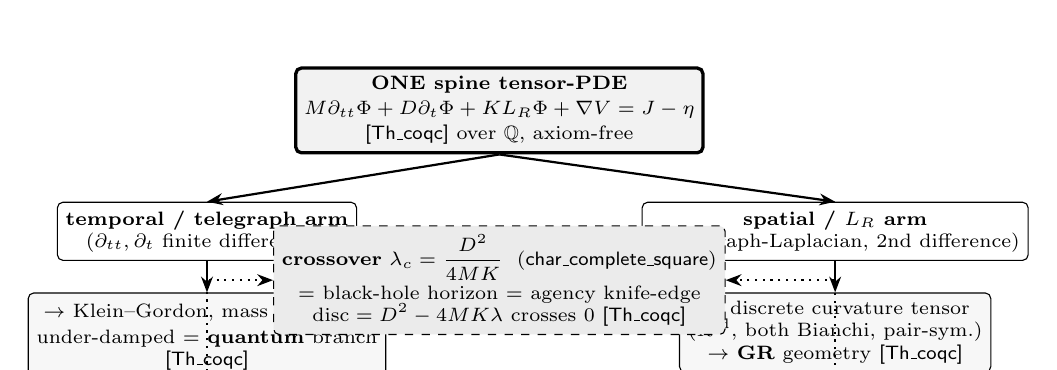
\begin{tikzpicture}[
  >={Stealth[length=2mm]},
  font=\scriptsize,
  spine/.style   ={draw,very thick,rounded corners=2pt,align=center,
                    inner sep=3pt,fill=black!5},
  arm/.style     ={draw,rounded corners=2pt,align=center,inner sep=3pt},
  readout/.style ={draw,rounded corners=2pt,align=center,inner sep=3pt,fill=black!3},
  edge/.style    ={draw,rounded corners=2pt,align=center,inner sep=3pt,
                    dashed,fill=black!8},
  link/.style    ={->,thick},
  node distance  =4mm and 4mm]

% --- central spine PDE ---
\node[spine] (spine) {\textbf{ONE spine tensor-PDE}\\[1pt]
  $M\partial_{tt}\Phi + D\partial_{t}\Phi + K\LR\Phi + \nabla V = J-\eta$\\[1pt]
  \textsf{[Th\_coqc]} over $\mathbb{Q}$, axiom-free};

% --- two arms ---
\node[arm,below left=6mm and -8mm of spine]  (tarm)
  {\textbf{temporal / telegraph arm}\\ ($\partial_{tt},\partial_{t}$ finite differences)};
\node[arm,below right=6mm and -8mm of spine] (sarm)
  {\textbf{spatial / $\LR$ arm}\\ (root graph-Laplacian, 2nd difference)};

\draw[link] (spine.south) -- (tarm.north);
\draw[link] (spine.south) -- (sarm.north);

% --- readouts at the ends of the arms ---
\node[readout,below=of tarm] (kg)
  {$\to$ Klein--Gordon, mass $M=\tfrac{1}{2\tau_c}$,\\
   under-damped $=$ \textbf{quantum} branch\\
   \textsf{[Th\_coqc]}};
\node[readout,below=of sarm] (gr)
  {$\to$ discrete curvature tensor\\
   ($R^{\mathrm{fd}}$, both Bianchi, pair-sym.)\\
   $\to$ \textbf{GR} geometry \textsf{[Th\_coqc]}};

\draw[link] (tarm.south) -- (kg.north);
\draw[link] (sarm.south) -- (gr.north);

% --- the single crossover knife-edge where the arms meet ---
\node[edge,below=9mm of spine] (edge)
  {\textbf{crossover} $\lambda_c=\dfrac{D^2}{4MK}$
   \;(\textsf{char\_complete\_square})\\[1pt]
   $=$ black-hole horizon $=$ agency knife-edge\\
   $\mathrm{disc}=D^2-4MK\lambda$ crosses $0$ \textsf{[Th\_coqc]}};

\draw[link,dotted] (kg.south) |- (edge.west);
\draw[link,dotted] (gr.south) |- (edge.east);

\end{tikzpicture}
\caption{The central claim in one picture. A single discrete tensor-PDE spine (top,
machine-checked over $\mathbb{Q}$) carries \emph{two} exact readout arms: the temporal
telegraph arm reads out Klein--Gordon dynamics, the rational mass $M=1/(2\tau_c)$, and the
under-damped quantum branch; the spatial $\LR$ arm reads out the division-free discrete
curvature tensor (both Bianchi identities, derived pair symmetry) and the gravitational
geometry. The two arms meet at one rational knife-edge $\lambda_c=D^2/(4MK)$ where the
telegraph discriminant crosses zero --- simultaneously the quantum$\leftrightarrow$classical
transition, the horizon of the audited core, and the agency threshold: one identity, three
readings. All boxes are \textsf{[Th\_coqc]} readouts (\code{coqc}~8.20.1, axiom-free); the
continuum limit of any arm is \emph{not} shown because it is \textsf{[Refused]}, not omitted
(\S\ref{sec:refusal}) --- a machine-checked non-readout, never left \textsf{[Open]}.}
\label{fig:spine}
\end{figure}


%% KEY-CLAIM RESULTS TABLE
% Headline key-claim table. Requires \usepackage{tabularx,booktabs} (already loaded).
% twocolumn-safe (table*, full \textwidth). Column Y = ragged-right flexible X.
% Every row carries exactly one tier tag + the Coq object that closes it.
% Author: Yaoharee Lahtee / OCSI.
\begin{table*}[t]
\centering\footnotesize
\begin{tabularx}{\textwidth}{@{}p{3.05cm}Y c p{5.1cm}@{}}
\toprule
Key claim & Machine-checked readout (headline) & Tier & Coq object (file $\cdot$ module) \\
\midrule
Spine $=$ telegraph $\to$ KG / mass
  & $M\partial_{tt}\Phi+D\partial_{t}\Phi+K\LR\Phi=0$ \emph{is} the telegraph equation;
    exact rational mass $M=1/(2\tau_c)$; $D\to0$ oscillatory (KG/quantum), $M\to0$ diffusive.
  & \Thq{}
  & \code{InfoSchrodinger.v} $\cdot$ core \code{InfoTelegraph} \\
Quantum $\leftrightarrow$ classical crossover $=$ horizon
  & $\mathrm{disc}=D^2-4MK\lambda$ crosses $0$ at $\lambda_c=D^2/(4MK)$
    (\code{char\_complete\_square}); this crossover \emph{is} the core horizon disc.\ and the
    agency knife-edge --- one $\lambda_c$, three readings.
  & \Thq{}
  & \code{InfoTelegraphCrossover\_attempt.v};\newline
    \code{InfoTelegraphHorizonUnification\_attempt.v} \\
Curvature chain: Riemann
  & Riemann $=$ finite second difference $=$ Heisenberg commutator; affine $\Rightarrow$ flat,
    non-affine witness $R^{\mathrm{fd}}=2\ne0$, plaquette $[X,Y]$ central.
  & \Thq{}
  & \code{InfoDiscreteRiemannCurvature\_attempt.v};\newline
    \code{InfoDiscreteRiemannCommutator\_attempt.v} \\
Curvature chain: both Bianchi
  & First (algebraic) Bianchi $=$ Jacobi identity, $ij$-antisym.; second (differential)
    $dF=0$ abelian, non-vacuous nonzero-curvature witness.
  & \Thq{}
  & \code{InfoMetricCompatibleCurvature\_attempt.v};\newline
    \code{InfoDiscreteSecondBianchi\_attempt.v} \\
Curvature chain: pair symmetry (derived)
  & $R_{ijkl}=R_{klij}$ \emph{derived}, not posited, from A1 ($ij$) $+$ A2 ($kl$) $+$ B1
    (first Bianchi); all four Riemann symmetries thus machine-checked.
  & \Thq{}
  & \code{InfoRiemannPairSymmetry\_attempt.v} $\cdot$ \code{pair\_symmetry} \\
Curvature chain: metric-derived
  & Levi-Civita $\Gamma^{2}{}_{12}=\tfrac12\,dw/w$ and $R_{1212}=-\tfrac14$ rational; needs
    only $g^{-1}$, no $\sqrt{g}$ (frame $\sqrt{g}$ proven a non-readout).
  & \Thq{}
  & \code{InfoMetricDerivedCurvature\_attempt.v};\newline
    \code{InfoMetricFrameNonReadout\_attempt.v} ($\to$\Refu{}) \\
Falsifiable $\tau_{\mathrm{rel}}$ floor
  & Bounded $\LR$-spectrum $\lambda\le\Lambda$ forces $\Gamma_{\mathrm{rel}}D\le K\Lambda$, i.e.\
    a hard floor $\tau_{\mathrm{rel}}\ge D/(K\Lambda)>0$; the unbounded continuum has \emph{none} ---
    one clean $\tau_{\mathrm{rel}}(E)$ curve decides (\S\ref{sec:prediction}).
  & \Thq{}
  & \code{InfoTauFloor} $\cdot$ \code{discrete\_rate\_ceiling}\newline
    / \code{continuum\_no\_floor} \\
\bottomrule
\end{tabularx}
\caption{The headline results in one ledger. Each row is a central claim of this paper, its
machine-checked readout, its single tier tag, and the Coq object that closes it (file names
are the \code{formal/*.v} sources of Table~\ref{tab:artifacts}; \code{InfoTelegraph} and
\code{InfoTauFloor} name the core modules that carry the mass identity and the rate-ceiling /
no-floor pair). Every headline is \Thq{} --- axiom-free over $\mathbb{Q}$, \code{coqc}~8.20.1
exit~0, \code{Print Assumptions} \emph{Closed under the global context}. The continuum limit of
any readout is \Refu{} (\S\ref{sec:refusal}), never \Open{}; the sole world-facing prediction
is the $\tau_{\mathrm{rel}}$ floor, whose falsifying datum and retraction are pre-committed
(\S\ref{sec:pred-retract}).}
\label{tab:keyclaims}
\end{table*}


\subsection{Discrete dynamics --- the actual update}\label{sec:spine-dyn}

Equation \eqref{eq:master} is not a shorthand for a continuum operator. On an
$\LR$-eigenmode of eigenvalue $\lambda$ and a lattice tick, $\partial_{tt}$ and
$\partial_{t}$ are finite differences and the field is advanced by an exact two-register
(position/velocity) update:
\begin{align}
X[n+1] &= X[n] + \Delta\theta_R\,V[n], \label{eq:updX}\\
V[n+1] &= V[n] + \frac{\Delta\theta_R}{M}\Bigl(K\,\LR\Phi - D\,V[n] \notag\\
  &\hphantom{{}= V[n] + \frac{\Delta\theta_R}{M}\Bigl(}{} - \nabla V(\Phi)
  + J - \eta\Bigr). \label{eq:updV}
\end{align}
Here $n\in\mathbb{N}$ is the tick counter and $\Delta\theta_R$ is the retained-distinction
phase increment --- \emph{not} a physical $dt$, and never the limit $dt\to 0$ (see the Clock
Registry, \S\ref{sec:clock}). Every register is a rational readout; no limit is taken. The
backward-Euler / decay-ratio form of the $D\,\partial_t$ piece is the core brick
\code{InfoDecayRatioFromTauC}; its continuum companion $\exp(-\Gamma_{\mathrm{damp}} t)$ is an $h\!\to\!0$
object (I2) and is \Refu{} (\S\ref{sec:refusal}). \Thq{}

\subsection{Action and Euler--Lagrange envelope}\label{sec:spine-action}

The update \eqref{eq:updX}--\eqref{eq:updV} is not posited; it is stationary for a discrete
window action, in the Euler--Lagrange first-variation lineage \cite{euler1744,lagrange1788};
the resulting two-register recurrence is exactly the St\"ormer--Verlet leapfrog integrator
\cite{stormer1907,verlet1967}. Over one node-window $p\to m\to q$,
\begin{equation}\label{eq:action}
A_{\mathrm{win}}(m) = M\,|q-m|^2 + M\,|m-p|^2 - h^2 K\,\mathrm{gform}(m,m),
\end{equation}
with linear coefficient $S_{\mathrm{geo}} = h^2 K\,\mathrm{gform}(m,m) - \sum_{e}
\mathrm{benefit}(e)$ and diagonal $C_i = 2M - h^2 K\,\mathrm{gdeg}(i)$. Stationarity
$\partial A_{\mathrm{win}}/\partial m = 0$ reproduces the discrete spine update exactly, as
a ring identity in $\mathbb{Q}$ --- no variation-in-the-limit is invoked
(\code{InfoActionStationarity}). The geodesic companion gives
$M\,\mathrm{acc} = \tfrac12\gamma\,\mathrm{vel}^2$ as the exact discretization of
$M\ddot{x} = -\tfrac12 M'\dot{x}^2$ (\code{InfoGeodesicActionStationarity}). \Thq{}

% =====================================================================
\section{Clock Registry}\label{sec:clock}
% =====================================================================

Time-like symbols are the classic site of silent substitution: a tick becomes a duration,
a phase increment becomes a metric interval, a limit is slipped in. We firewall every
time-like symbol in Table~\ref{tab:clock}. The rule is one line: \emph{no symbol below is
silently substituted for another, and each equation states which clock it runs on}. \Dr{}

\begin{table*}[t]
\centering\footnotesize
\begin{tabularx}{\textwidth}{@{}llYY@{}}
\toprule
Symbol & Name & What it is & Must not be confused with \\
\midrule
$n$ & tick index & dimensionless counter of update steps ($\mathbb{N}$) &
  physical elapsed time $t$; a duration \\
$\Delta\theta_R$ & retained-distinction phase increment & the per-tick advance in
  \eqref{eq:updX}--\eqref{eq:updV} & a physical $dt$; a metric interval \\
$\tau_c$ & correlation / agency time & the retained-distinction correlation scale; the mass
  constant, $M=1/(2\tau_c)$ & $\tau_{\mathrm{rel}}$ (eigenmode relaxation time); $\tau_R$; the horizon $\lambda_c$; wall-clock $t$ \\
$dt$ & observer step & a chosen finite readout step (backward-Euler in
  \code{InfoDecayRatioFromTauC}) & $\Delta\theta_R$; the continuum limit $dt\to 0$ (\Refu{}) \\
$t$ & physical time & the interpretive elapsed-time readout $t=n\cdot dt$ &
  the tick index $n$; $\Delta\theta_R$ \\
$\Gamma_{\mathrm{damp}}$ & damping rate & the dissipative rate $\Gamma_{\mathrm{damp}}=D/(2M)$ (over-damped exponent) &
  $\Gamma_{\mathrm{rel}}$; $\tau_c$; $\lambda_c$; a frequency $\omega$ \\
$\Gamma_{\mathrm{rel}}(\lambda)$ & eigenmode relaxation rate & the per-mode relaxation rate $\Gamma_{\mathrm{rel}}=K\lambda/D$ (\S\ref{sec:prediction}) &
  $\Gamma_{\mathrm{damp}}=D/(2M)$; the mass scale $\tau_c$ \\
$\tau_{\mathrm{rel}}(\lambda)$ & eigenmode relaxation time & the per-mode relaxation time $\tau_{\mathrm{rel}}=1/\Gamma_{\mathrm{rel}}=D/(K\lambda)$; floored by a bounded spectrum &
  $\tau_c$ (the mass scale, $M=1/(2\tau_c)$); $\tau_R$; the horizon $\lambda_c$ \\
$\tau_R$ & readout / refresh time & the observer's readout cadence &
  $\tau_c$ (a system property, not the observer's) \\
$\omega$ & mode frequency & the temporal characteristic root of $M\omega^2+D\omega+K\lambda=0$ &
  $\Gamma_{\mathrm{damp}}$ (decay) --- the sign of the discriminant decides which \\
\bottomrule
\end{tabularx}
\caption{Clock Registry. Every time-like symbol in the paper, with what it is and the
symbols it must never be silently swapped for. The continuum limit $dt\to 0$ appears only as
an explicitly \Refu{} object.}
\label{tab:clock}
\end{table*}

% =====================================================================
\section{Node Registry}\label{sec:nodes}
% =====================================================================

Table~\ref{tab:nodes} lists the chain as a registry of nodes: each an equation or object,
with its file/theorem, its tier, and the gate it must pass. The flow is
\emph{difference $\to$ $\LR$ $\to$ spine $\to$ telegraph $\to$ crossover $\to$ horizon $\to$
curvature $\to$ Bianchi}. Every node but the last-listed frame refusal is \Thq{}; N14 is a
\Thq{} theorem \emph{that} the $\sqrt{g}$ frame is a non-readout, i.e.\ a verified refusal.

\begin{table*}[t]
\centering\footnotesize
{\renewcommand{\code}[1]{\texttt{\seqsplit{#1}}}%
\begin{tabularx}{\textwidth}{@{}lYYlY@{}}
\toprule
Node & Object / equation & File $\cdot$ theorem & Tier & Gate \\
\midrule
N1 difference & $\mathrm{christoffel\_fd}\,w\,j = w(Sj)-w(j)$ &
  \code{InfoDiscreteRiemannCurvature} $\cdot$ \code{riemann\_is\_second\_difference} & \Thq{} &
  exact ring identity, no $h\!\to\!0$ \\
N2 $\LR$ & root graph-Laplacian $=$ second difference of the field &
  core; $\mathrm{riemann\_fd}=w(SSj)-2w(Sj)+w(j)$ & \Thq{} & axiom-free; the spatial-geometry axis \\
N3 spine & $M\partial_{tt}\Phi+D\partial_t\Phi+K\LR\Phi=0$ &
  \code{InfoSchrodinger}/\code{InfoDecoherence}/\code{InfoTelegraph} & \Thq{} &
  three readouts of one equation \\
N4 telegraph & spine \textbf{is} telegraph, $M=1/(2\tau_c)$ &
  core \code{InfoTelegraph} & \Thq{} & mass identity exact over $\mathbb{Q}$ \\
N5 crossover & $\mathrm{disc}=D^2-4MK\lambda$; $\lambda_c=D^2/(4MK)$ &
  \code{InfoTelegraphCrossover} $\cdot$ \code{char\_complete\_square} & \Thq{} &
  completion-of-square exact; both signs witnessed \\
N6 horizon & telegraph disc $=$ core horizon disc; crossover $=$ agency edge &
  \code{InfoTelegraphHorizonUnification} $\cdot$ \code{disc\_is\_spine\_discr} & \Thq{} &
  identity to core \code{InfoFrontier.spine\_discr} \\
N7 curvature (scalar) & affine $\Rightarrow$ flat; Christoffel $\ne$ curvature &
  \code{InfoDiscreteRiemannCurvature} $\cdot$ \code{affine\_is\_flat} & \Thq{} &
  non-affine witness $\mathrm{riemann\_fd}=2\ne 0$ \\
N8 curvature (2-index) & $R_{xy}=$ center of $[X,Y]=a\cdot b$ (Heisenberg, division-free) &
  \code{InfoDiscreteRiemannCommutator} $\cdot$ \code{plaquette\_curvature\_z} & \Thq{} &
  abelian/scalar/same-dir flat; $kl$-antisym exact \\
N9 metric-compatible & $\mathfrak{so}(3)$ generator antisym; $[\mathrm{asym}\,u,\mathrm{asym}\,w]=\mathrm{asym}(u\times w)$; Jacobi $=$ 1st Bianchi &
  \code{InfoMetricCompatibleCurvature} $\cdot$ \code{bianchi\_jacobi} & \Thq{} &
  $ij$-antisym + algebraic Bianchi, division-free \\
N10 rational isometry & $SO(2)$ Cayley $N^{\!\top}N=(1+t^2)^2 I$; $SO(3)$ holonomy $\ne I$ &
  \code{InfoRationalIsometry}, \code{InfoRationalSO3Curvature} & \Thq{} &
  rational orthogonal transport, no $\sqrt{\ }$ \\
N11 metric-derived & Levi-Civita $\Gamma^{2}{}_{12}=\tfrac12\,dw/w$ rational; $R_{1212}$ rational &
  \code{InfoMetricDerivedCurvature} $\cdot$ \code{christoffel\_G212\_rational} & \Thq{} &
  needs only $g^{-1}$ (rational); no $\sqrt{g}$ \\
N12 Bianchi (differential) & abelian $dF=0$: $d_z F_{xy}+d_x F_{yz}+d_y F_{zx}=0$ &
  \code{InfoDiscreteSecondBianchi} $\cdot$ \code{second\_bianchi} & \Thq{} &
  nonzero-curvature witness (non-vacuous) \\
N13 pair symmetry & $R_{ijkl}=R_{klij}$ \emph{derived} from A1+A2+B1 &
  \code{InfoRiemannPairSymmetry} $\cdot$ \code{pair\_symmetry} & \Thq{} &
  derived, not posited; abstract $R$ \\
N14 frame refusal & $\sqrt{g}$ orthonormal frame is an I1 non-readout &
  \code{InfoMetricFrameNonReadout} $\cdot$ \code{metric\_frame\_diag12\_no\_rational} &
  \Thq{}$\to$\Refu{} & connection stays rational; only $\sqrt{g}$ refused \\
N15 non-abelian defect & naive covariant Bianchi fails by $\times(dA,dB)$ &
  \code{InfoDiscreteLeibnizObstruction} & \Thq{} &
  exact Leibniz defect (honest negative) \\
\bottomrule
\end{tabularx}}
\caption{Node Registry. Each row is one object in the chain with the theorem that closes it
and the gate it passes. N1--N13 and N15 are \Thq{} positive/negative results over
$\mathbb{Q}$; N14 is a \Thq{} theorem \emph{that} the $\sqrt{g}$ frame is a non-readout,
i.e.\ a verified refusal, and is routed to \S\ref{sec:refusal}.}
\label{tab:nodes}
\end{table*}

% =====================================================================
\section{The telegraph discriminant crossover: quantum $\leftrightarrow$ classical
  $=$ horizon $=$ agency knife-edge}\label{sec:crossover}
% =====================================================================

The temporal characteristic of the spine \eqref{eq:spine} on an $\LR$-eigenmode $\lambda$ is
\begin{equation}\label{eq:pchar}
\mathrm{pchar}(\omega) = M\omega^2 + D\omega + K\lambda,\quad
\mathrm{disc} = D^2 - 4MK\lambda,
\end{equation}
with crossover $\lambda_c = D^2/(4MK)$. The entire crossover is carried by one algebraic
identity, the completion of the square:
\begin{equation}\label{eq:complete}
\begin{aligned}
4M\cdot\mathrm{pchar}(\omega) &= (2M\omega + D)^2 - \mathrm{disc}\\
&\quad(\code{char\_complete\_square},\ \Thq{}).
\end{aligned}
\end{equation}
The crossover, its two regimes, and the knife-edge $\lambda_c$ are drawn in
Figure~\ref{fig:crossover}.

%% CROSSOVER SCHEMATIC
% Telegraph discriminant crossover schematic: disc(lambda)=D^2-4MK lambda vs the
% L_R eigenvalue lambda, splitting under-damped/oscillatory (quantum) from
% over-damped/decay (classical) at the single knife-edge lambda_c = D^2/(4MK).
% Requires \usepackage{tikz}; \usetikzlibrary{positioning,arrows.meta} (already loaded).
% Single-column figure (twocolumn-safe). Author: Yaoharee Lahtee / OCSI.
\begin{figure}[t]
\centering
\resizebox{\columnwidth}{!}{%
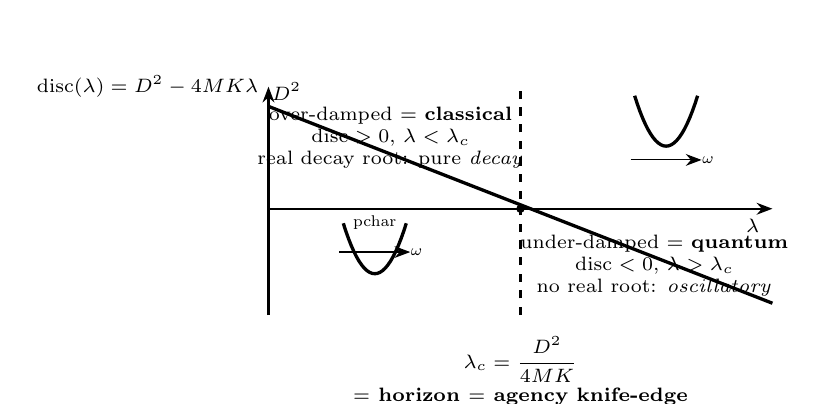
\begin{tikzpicture}[
  >={Stealth[length=2mm]},
  font=\scriptsize,
  axisline/.style={draw,thick,->},
  discline/.style={draw,very thick},
  crit/.style={draw,dashed,thick},
  reg/.style={align=center,inner sep=1pt},
  inset/.style={draw,rounded corners=2pt,inner sep=2pt,fill=black!3}]

% --- axes: horizontal lambda, vertical disc ---
\def\W{6.4}   % lambda-axis length
\def\LC{3.2}  % lambda_c position on the axis
\coordinate (O) at (0,0);
\draw[axisline] (O) -- (\W,0) node[below left=0pt and 1pt]{$\lambda$};
\draw[axisline] (0,-1.35) -- (0,1.55) node[left]{$\mathrm{disc}(\lambda)=D^2-4MK\lambda$};

% --- the descending discriminant line: disc = D^2 - 4MK lambda, zero at lambda_c ---
% slope chosen so the line spans +1.3 at lambda=0 down to -1.2 at lambda=W.
\coordinate (L0) at (0,1.3);      % disc(0)=D^2 > 0
\coordinate (Lend) at (\W,-1.2);  % disc large lambda < 0
\draw[discline] (L0) -- (Lend);
\node[above right=1pt and 0pt of L0,inner sep=1pt] {$D^2$};

% --- critical eigenvalue: vertical knife-edge at lambda_c ---
\draw[crit] (\LC,-1.35) -- (\LC,1.55);
\filldraw (\LC,0) circle (1.3pt);
\node[align=center,anchor=north] at (\LC,-1.5)
  {$\lambda_c=\dfrac{D^2}{4MK}$\\[1pt]
   \textbf{$=$ horizon $=$ agency knife-edge}};

% --- regime labels ---
\node[reg] at (1.55,0.9)  {over-damped $=$ \textbf{classical}\\ $\mathrm{disc}>0$, $\lambda<\lambda_c$\\ real decay root: pure \emph{decay}};
\node[reg] at (4.9,-0.72) {under-damped $=$ \textbf{quantum}\\ $\mathrm{disc}<0$, $\lambda>\lambda_c$\\ no real root: \emph{oscillatory}};

% --- inset A: over-damped parabola pchar(omega) dips below axis (real roots) ---
\begin{scope}[shift={(1.35,-0.55)},scale=0.5]
  \draw[->] (-0.9,0) -- (0.9,0) node[right,inner sep=0pt,scale=0.8]{$\omega$};
  \draw[very thick] plot[domain=-0.8:0.8,samples=25] (\x,{2*\x*\x-0.55});
  \node[scale=0.8] at (0,0.75) {$\mathrm{pchar}$};
\end{scope}

% --- inset B: under-damped parabola floats above axis (no real root) ---
\begin{scope}[shift={(5.05,0.62)},scale=0.5]
  \draw[->] (-0.9,0) -- (0.9,0) node[right,inner sep=0pt,scale=0.8]{$\omega$};
  \draw[very thick] plot[domain=-0.8:0.8,samples=25] (\x,{2*\x*\x+0.35});
\end{scope}

\end{tikzpicture}%
}
\caption{The telegraph discriminant crossover, drawn from the completion-of-square
identity $4M\,\mathrm{pchar}(\omega)=(2M\omega+D)^2-\mathrm{disc}$ (\code{char\_complete\_square}).
The discriminant $\mathrm{disc}(\lambda)=D^2-4MK\lambda$ (heavy line) falls monotonically
in the $\LR$-eigenvalue $\lambda$ and crosses zero at the single critical value
$\lambda_c=D^2/(4MK)$ (\code{critical\_disc\_zero}). Left of the knife-edge
($\lambda<\lambda_c$, $\mathrm{disc}>0$) the characteristic $\mathrm{pchar}(\omega)=M\omega^2+D\omega+K\lambda$
dips to a non-positive minimum (inset, lower left), so a real decay root exists and the
mode purely \emph{decays} --- the over-damped, diffusive, \textbf{classical} branch
(\code{overdamped\_min\_nonpositive}). Right of it ($\lambda>\lambda_c$, $\mathrm{disc}<0$)
$\mathrm{pchar}$ stays strictly positive (inset, upper right), so there is no real
frequency root and the mode is \emph{oscillatory} --- the under-damped, wave,
\textbf{quantum} branch (\code{underdamped\_positive}, \code{underdamped\_iff\_above\_crit}).
The same rational $\lambda_c$ is simultaneously the quantum$\leftrightarrow$classical
transition, the horizon of the audited core (\code{disc\_is\_spine\_discr},
\code{InfoTelegraphHorizonUnification}), and the agency threshold: one identity, three
readings. Both regimes and the edge are \textsf{[Th\_coqc]} over $\mathbb{Q}$ (\code{coqc}
8.20.1, axiom-free); the crossover curve is a schematic of those exact readouts, not a
fitted plot.}
\label{fig:crossover}
\end{figure}


From \eqref{eq:complete} the two regimes and the edge follow exactly over $\mathbb{Q}$:
\begin{itemize}\itemsep2pt
\item \textbf{Under-damped $=$ quantum} ($\mathrm{disc}<0$): $\mathrm{pchar}(\omega)>0$ for
  every real $\omega$, so there is no real frequency root and the mode is oscillatory ---
  the wave/quantum (\code{InfoSchrodinger}) side (\code{underdamped\_positive}). \Thq{}
\item \textbf{Over-damped $=$ classical} ($\mathrm{disc}\ge 0$): $\mathrm{pchar}(\omega)\le 0$
  at $\omega=-D/2M$, so a real decay root exists and the mode purely decays --- the
  diffusive/classical (\code{InfoDecoherence}) side
  (\code{overdamped\_min\_nonpositive}). \Thq{}
\item \textbf{Crossover / critical damping}: $\mathrm{disc}(\lambda_c)=0$ at
  $\lambda_c=D^2/(4MK)$ (\code{critical\_disc\_zero}); and $\mathrm{disc}<0 \iff D^2<4MK\lambda$,
  i.e.\ $\lambda$ above $\lambda_c$ (\code{underdamped\_iff\_above\_crit}). \Thq{}
\item \textbf{Witnesses}: $(M,D,K,\lambda)=(1,1,1,1)\Rightarrow \mathrm{disc}=-3<0$
  (under-damped/quantum); $(1,4,1,1)\Rightarrow \mathrm{disc}=12>0$
  (over-damped/classical). \Fin{}
\end{itemize}

\paragraph{One knife-edge, three readings.} The telegraph discriminant \eqref{eq:pchar}
\emph{is} the audited core's \code{InfoFrontier.spine\_discr}, and $\lambda_c$ \emph{is}
\code{spine\_lambda\_c}; the oscillatory (quantum) regime is exactly the region above the
horizon (\code{disc\_is\_spine\_discr}, \code{lam\_c\_is\_spine\_lambda\_c},
\code{quantum\_iff\_above\_horizon}, \code{oscillatory\_above\_horizon},
\code{InfoTelegraphHorizonUnification}). \Thq{}. The reading: a single rational knife-edge
$\lambda_c$ unifies the quantum$\leftrightarrow$classical transition (dynamics), the
black-hole horizon (the geometric side of the core), and the agency threshold ---
looping/quantum above it, settling/classical at or below it. \Dr{}

% =====================================================================
\section{The discrete curvature-tensor chain}\label{sec:curvature}
% =====================================================================

The geometry operator $\LR$ in \eqref{eq:master} is the entry point to a full discrete
curvature calculus, division-free and exact over $\mathbb{Q}$. Every object below is the
discrete analogue of a classical construction of Riemannian geometry --- the Christoffel
symbols \cite{christoffel1869}, the Riemann curvature tensor \cite{riemann1868}, the Bianchi
identities \cite{bianchi1902}, and the curvature--holonomy relation of Gauss and Bonnet
\cite{gauss1828,bonnet1848} --- but each is reproduced here as an exact rational readout.
Every step is \Thq{}. The chain and its inter-node dependencies, each labelled with the
Coq file that closes it, are drawn as a DAG in Figure~\ref{fig:curvature-dag}.

%% CURVATURE-CHAIN DEPENDENCY DAG
% Discrete curvature-chain dependency DAG. Each node is one object in the
% division-free rational curvature calculus, labelled with the Coq file that closes it.
% Requires \usepackage{tikz}; \usetikzlibrary{positioning,arrows.meta} (already loaded).
% Full-width figure* (twocolumn-safe: spans both columns). Author: Yaoharee Lahtee / OCSI.
\begin{figure*}[t]
\centering
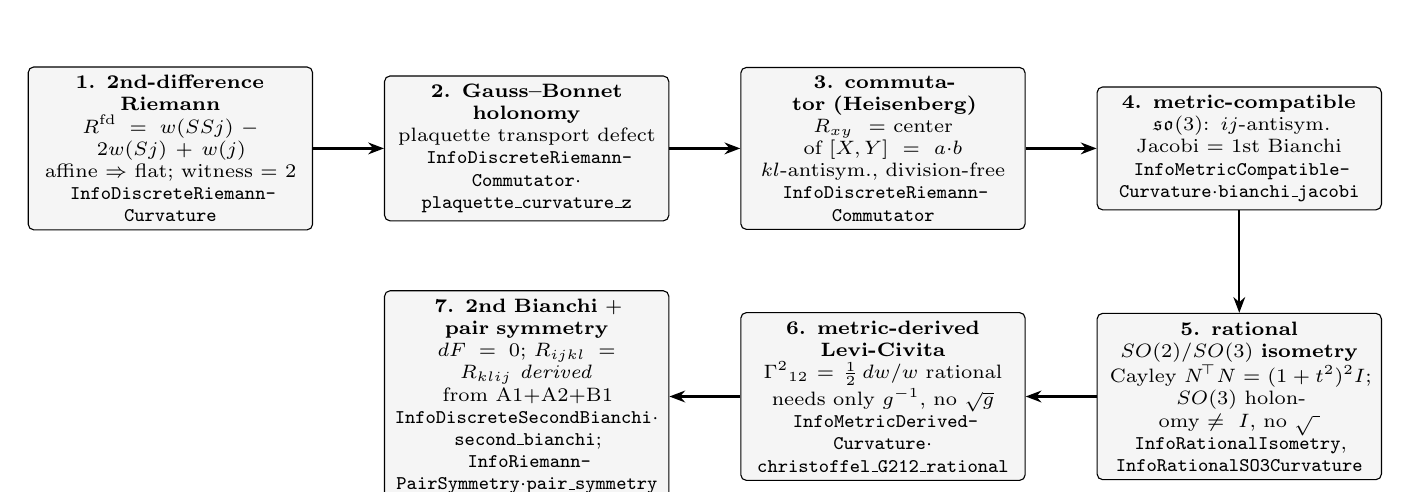
\begin{tikzpicture}[
  >={Stealth[length=2mm]},
  font=\scriptsize,
  cnode/.style={draw,rounded corners=2pt,align=center,inner sep=3pt,
                fill=black!4,text width=34mm,minimum height=11mm},
  link/.style={->,thick},
  node distance=6mm and 9mm]

% --- the chain, left to right, with two branch merges ---
\node[cnode] (n1)
  {\textbf{1. 2nd-difference Riemann}\\
   $R^{\mathrm{fd}}=w(SSj)-2w(Sj)+w(j)$\\
   affine $\Rightarrow$ flat; witness $=2$\\
   {\ttfamily InfoDiscreteRiemann-}\\{\ttfamily Curvature}};

\node[cnode,right=of n1] (n2)
  {\textbf{2. Gauss--Bonnet holonomy}\\
   plaquette transport defect\\
   {\ttfamily InfoDiscreteRiemann-}\\{\ttfamily Commutator}$\cdot$\\{\ttfamily plaquette\_curvature\_z}};

\node[cnode,right=of n2] (n3)
  {\textbf{3. commutator (Heisenberg)}\\
   $R_{xy}=$ center of $[X,Y]=a{\cdot}b$\\
   $kl$-antisym., division-free\\
   {\ttfamily InfoDiscreteRiemann-}\\{\ttfamily Commutator}};

\node[cnode,right=of n3] (n4)
  {\textbf{4. metric-compatible}\\
   $\mathfrak{so}(3)$: $ij$-antisym.\\
   Jacobi $=$ 1st Bianchi\\
   {\ttfamily InfoMetricCompatible-}\\{\ttfamily Curvature}$\cdot${\ttfamily bianchi\_jacobi}};

% second row (below), continuing the chain
\node[cnode,below=13mm of n4] (n5)
  {\textbf{5. rational $SO(2)/SO(3)$ isometry}\\
   Cayley $N^{\!\top}N=(1+t^2)^2 I$;\\
   $SO(3)$ holonomy $\ne I$, no $\sqrt{\ }$\\
   {\ttfamily InfoRationalIsometry},\\{\ttfamily InfoRationalSO3Curvature}};

\node[cnode,left=of n5] (n6)
  {\textbf{6. metric-derived Levi-Civita}\\
   $\Gamma^{2}{}_{12}=\tfrac12\,dw/w$ rational\\
   needs only $g^{-1}$, no $\sqrt{g}$\\
   {\ttfamily InfoMetricDerived-}\\{\ttfamily Curvature}$\cdot$\\{\ttfamily christoffel\_G212\_rational}};

\node[cnode,left=of n6] (n7)
  {\textbf{7. 2nd Bianchi $+$ pair symmetry}\\
   $dF=0$; $R_{ijkl}=R_{klij}$ \emph{derived}\\
   from A1$+$A2$+$B1\\
   {\ttfamily InfoDiscreteSecondBianchi}$\cdot$\\{\ttfamily second\_bianchi};
   {\ttfamily InfoRiemann-}\\{\ttfamily PairSymmetry}$\cdot${\ttfamily pair\_symmetry}};

% --- dependency arrows ---
\draw[link] (n1) -- (n2);
\draw[link] (n2) -- (n3);
\draw[link] (n3) -- (n4);
\draw[link] (n4.south) -- (n5.north);   % turn down into second row
\draw[link] (n5) -- (n6);
\draw[link] (n6) -- (n7);

\end{tikzpicture}
\caption{The discrete curvature-tensor chain as a dependency DAG, division-free and exact
over $\mathbb{Q}$, each node labelled with the Coq file (and where sharp, the theorem) that
closes it. The chain runs: (1) Riemann as an exact second difference (affine $\Rightarrow$
flat, with a non-vacuous curved witness $R^{\mathrm{fd}}=2$); (2) the plaquette holonomy /
discrete Gauss--Bonnet transport defect; (3) the same curvature as a Heisenberg commutator
$R_{xy}=$ center of $[X,Y]=a{\cdot}b$, giving genuine two-index, $kl$-antisymmetric structure
in the nilpotent center; (4) metric compatibility on $\mathfrak{so}(3)\cong(\mathbb{Q}^3,\times)$,
where $ij$-antisymmetry holds and the Jacobi identity \emph{is} the first (algebraic) Bianchi
identity; (5) a rational $SO(2)/SO(3)$ isometry group via the Cayley transform, with a
holonomy-$\ne I$ $SO(3)$ capstone and no square roots; (6) the metric-derived Levi-Civita
connection $\Gamma^{2}{}_{12}=\tfrac12\,dw/w$, needing only $g^{-1}$ and never $\sqrt{g}$; and
(7) the second (differential) Bianchi identity together with the pair symmetry
$R_{ijkl}=R_{klij}$ \emph{derived}, not posited, from the two antisymmetries and the first
Bianchi. All four Riemann symmetries and both Bianchi identities are thus machine-checked;
the chain is structurally complete over $\mathbb{Q}$. Every node is \textsf{[Th\_coqc]}
(\code{coqc} 8.20.1, axiom-free); the $\sqrt{g}$ orthonormal frame the chain deliberately
avoids is \textsf{[Refused]} as a non-readout, never left \textsf{[Open]}
(\S\ref{sec:refusal}).}
\label{fig:curvature-dag}
\end{figure*}


\paragraph{1. Christoffel as first difference.} $\mathrm{christoffel\_fd}\,w\,j = w(Sj)-w(j)$
(the discrete Christoffel symbol \cite{christoffel1869}).
An affine weight gives a nonzero Christoffel ($=b$) yet zero curvature: Christoffel $\ne$
curvature, exactly (\code{christoffel\_can\_be\_nonzero\_while\_flat}).

\paragraph{2. Riemann as second difference.} (the discrete Riemann tensor
\cite{riemann1868})
$\mathrm{riemann\_fd} = w(SSj) - 2w(Sj) + w(j)$; affine $\Rightarrow$ flat; the non-affine
witness $w=q n^2$ gives $\mathrm{riemann\_fd}\,0 = 2\ne 0$; and flat $\iff$ locally affine
(arithmetic progression) (\code{riemann\_is\_second\_difference}, \code{affine\_is\_flat},
\code{curvature\_nonzero\_witness}, \code{flat\_iff\_second\_diff\_zero}).

\paragraph{3. Riemann as commutator (genuinely 2-index).} On the Heisenberg /
upper-unipotent group with polynomial (division-free) inverse --- curvature as the
non-commutation of transport, a matrix-mechanics commutator \cite{bornjordan1925} and, around a
plaquette, a discrete Gauss--Bonnet holonomy \cite{gauss1828,bonnet1848} --- $R_{xy}$ is the
center of $[X,Y]=a\cdot b$, with $[Y,X]=-a\cdot b$ ($kl$-antisymmetry, exact in the nilpotent center);
abelian, scalar, and same-direction cases are all flat, strictly exceeding the scalar brick
(\code{plaquette\_curvature\_z}, \code{reverse\_antisymmetric}, \code{curvature\_is\_central}).

\paragraph{4. First (algebraic) Bianchi and $ij$-antisymmetry.} Metric-compatible
$\mathfrak{so}(3)\cong(\mathbb{Q}^3,\times)$: the generator $\mathrm{asym}\,u$ is
antisymmetric, the matrix commutator is $\mathrm{asym}(u\times w)$ (so $\mathfrak{so}(3)$ is
closed under bracket), curvature is $ij$-antisymmetric, and the Jacobi identity \emph{is} the
first (algebraic) Bianchi identity \cite{bianchi1902} (\code{asym\_is\_antisymmetric},
\code{commutator\_is\_asym\_cross},
\code{curvature\_ij\_antisymmetric}, \code{bianchi\_jacobi}).

\paragraph{5. Second (differential) Bianchi.} \cite{bianchi1902} On the 3-D lattice,
abelian $dF=0$:
$d_z F_{xy} + d_x F_{yz} + d_y F_{zx} = 0$, from mixed-difference commutation, with a
nonzero-curvature witness so the identity is non-vacuous (\code{second\_bianchi},
\code{mixed\_differences\_commute}).

\paragraph{6. Pair symmetry, derived.} $R_{ijkl}=R_{klij}$ is \emph{derived} --- not
posited --- from A1 ($ij$-antisymmetry) $+$ A2 ($kl$-antisymmetry) $+$ B1 (first Bianchi),
for abstract $R$ over $\mathbb{Q}$, via the classical four-Bianchi-sum argument
(\code{pair\_symmetry}). All four Riemann symmetries are thus machine-checked.

\paragraph{7. Metric-derived Levi-Civita (rational).} $\Gamma^{2}{}_{12}=\tfrac12\,dw/w$ is
rational for $w\ne 0$ (needing only $g^{-1}$, no $\sqrt{g}$, no I1); $R_{1212} = -\tfrac12\,
d^2 w + (dw)^2/(4w)$; flat on constant $w$, curved witness $R_{1212}=-\tfrac14$
(\code{christoffel\_G212\_rational}, \code{flat\_constant\_zero\_curvature},
\code{curved\_witness}).

\paragraph{8. Rational isometry group.} $SO(2)$ exists over $\mathbb{Q}$ via the
Cayley/Pythagorean transform \cite{cayley1846} $N^{\!\top}N=(1+t^2)^2 I$; a rational $SO(3)$ capstone (two
$(3,4,5)$ rotations, holonomy $\ne I$) gives nonzero rational curvature, division-free
(\code{InfoRationalIsometry}, \code{InfoRationalSO3Curvature}).

All four Riemann symmetries ($kl$-antisymmetry, $ij$-antisymmetry, first Bianchi, pair
symmetry) and both Bianchi identities are machine-checked; the discrete curvature chain is
\emph{structurally complete} over $\mathbb{Q}$. \Thq{}

% =====================================================================
\section{Continuum Refusal}\label{sec:refusal}
% =====================================================================

A continuum-seeking discrete-gravity programme poses a graph-to-continuum gate (G7,
Table~\ref{tab:gates}): does the discrete theory converge to a smooth tensor field? \textbf{We
delete that gate and replace it with a Continuum Refusal.} The discrete tensor PDE over
$\mathbb{Q}$ (\S\ref{sec:spine}) \emph{is} the theory; there is no smooth limit to reach, and
reaching one is not a success criterion. \Refu{} (thesis).

The diagnosis is readout-not-truth: every continuum object the deleted gate would demand is
an \emph{injected infinity}, and therefore a non-readout that an agency of finite means never
returns.
\begin{itemize}\itemsep2pt
\item \textbf{I1 ($\mathbb{R}$-completeness)} --- the smooth field; the orthonormal frame
  $\sqrt{g}$. Proven refused: the rational metric $\mathrm{diag}(1,2)$ has \emph{no} rational
  frame, so $\sqrt{g}$ is I1, while the connection and curvature stay rational readouts
  (\code{InfoMetricFrameNonReadout} $\cdot$ \code{metric\_frame\_diag12\_no\_rational}). \Thq{}$\to$\Refu{}
\item \textbf{I2 ($h\!\to\!0$ / Taylor limit)} --- continuum $d^2 g$, $d\Gamma$, the
  exponential $\exp(-\Gamma_{\mathrm{damp}} t)$. Our second difference and backward-Euler are the finite
  readouts; the limit is declined (\code{InfoDecayRatioFromTauC}). \Refu{}
\item \textbf{I3/I4 ($\mathrm{Re}\to\infty$, $+\infty$ tails)} --- not invoked; refused where
  they would appear. \Refu{}
\end{itemize}

The Continuum Refusal is a \emph{position, verified where it bites}, not an unmet goal. We
never say the theory ``converges to'' or ``should reproduce'' a continuum tensor PDE. The
discrete PDE is complete on its own terms; the continuum is the map, not the territory.
Crucially, refusal is not a synonym for open. An I1 object like $\sqrt{g}$ is not a theorem
we have failed to prove --- we have proven it is not a rational readout, and we decline it on
principle. This is the single most important distinction in the paper, and \S\ref{sec:remainder}
keeps it strictly apart from the genuine open work.

% =====================================================================
\section{The decisive falsifiable prediction: a $\tau_{\mathrm{rel}}$ floor from a bounded spectrum}
\label{sec:prediction}
% =====================================================================

This is the tier-jump. Everything up to here is an \emph{internal} theorem about a
discrete kernel; here the discrete kernel forces a statement about the \emph{world}
that the continuum cannot make, that has the opposite sign, and that a single clean
measurement decides. We do not hide behind ``interpretation'': we write the inequality,
we name the arenas, and we pre-commit to the retraction that a violating datum compels.

% ---------------------------------------------------------------------
\subsection{The structure: discreteness $\Rightarrow$ a rate ceiling $\Leftrightarrow$
  a relaxation-time floor}\label{sec:pred-structure}

Our framework lives on a \emph{discrete} graph --- atomicity / retained distinction is the
root, so the readout operator $\LR$ acts on a finite (or locally finite) index set. A
finite symmetric $\LR$ has a \emph{bounded} spectrum: every eigenvalue obeys
\begin{equation}\label{eq:gershgorin}
0 \;\le\; \lambda \;\le\; \Lambda,\qquad
\Lambda \;\le\; 2\,\max_i \deg(i)
\end{equation}
by Gershgorin's circle theorem \cite{gershgorin1931} --- the largest $\LR$-eigenvalue is
capped by twice the maximum node degree (sharpened by the Anderson--Morley bound
\cite{andersonmorley1985}). Atomicity is not a decorative postulate here: it is exactly the
hypothesis $\lambda\le\Lambda$.

On an $\LR$-eigenmode the spine \eqref{eq:spine} gives an \emph{eigenmode relaxation rate}
$\Gamma_{\mathrm{rel}}(\lambda)$ obeying $\Gamma_{\mathrm{rel}}\, D = K\lambda$, and a corresponding
\emph{eigenmode relaxation time} $\tau_{\mathrm{rel}}(\lambda) = 1/\Gamma_{\mathrm{rel}} = D/(K\lambda)$.
This relaxation time is a property of the bounded-spectrum mode; it is \emph{not} the
correlation/agency time $\tau_c=1/(2M)$ of the Clock Registry (\S\ref{sec:clock}), nor the
damping rate $\Gamma_{\mathrm{damp}}=D/(2M)$, and the three must not be conflated. Feeding the
bounded spectrum \eqref{eq:gershgorin} into $\Gamma_{\mathrm{rel}} D = K\lambda$ yields, exactly
over $\mathbb{Q}$, a \emph{ceiling} on the relaxation rate and therefore a \emph{positive floor}
on the eigenmode relaxation time:
\begin{equation}\label{eq:floor}
\boxed{\;\Gamma_{\mathrm{rel}} \;\le\; \frac{K\Lambda}{D}
\quad\Longleftrightarrow\quad
\tau_{\mathrm{rel}} \;=\; \frac{D}{K\lambda}\;\ge\;\frac{D}{K\Lambda}\;>\;0\;}
\end{equation}
The ceiling half is machine-checked with no axioms:

\begin{theorem}[Discrete rate ceiling / $\tau_{\mathrm{rel}}$ floor, \Thq{}]\label{thm:ceiling}
For rationals $\Gamma_{\mathrm{rel}},\lambda,\Lambda,K,D$ with $\Gamma_{\mathrm{rel}} D = K\lambda$, $\lambda\le\Lambda$
and $K\ge 0$, one has $\Gamma_{\mathrm{rel}} D \le K\Lambda$
\emph{(\code{InfoTauFloor.discrete\_rate\_ceiling})}. Consequently a bounded discrete
spectrum bounds the energy as well, $E^2M \le \hbar^2 K\Lambda$
\emph{(\code{InfoHypothesisSeeds.energy\_uv\_bounded})}: the same atomicity that floors
$\tau_{\mathrm{rel}}$ is the built-in UV cutoff.
\end{theorem}

The floor is not a soft ``typical scale''; it is a hard lower bound that holds
\emph{no matter how hard the system is driven}, because $\Lambda$ is fixed by the graph,
not by the drive.

% ---------------------------------------------------------------------
\subsection{The continuum has no floor --- the two are mutually exclusive}
\label{sec:pred-continuum}

The continuum quantum speed limit (Mandelstam--Tamm \cite{mandelstamtamm1945} /
Margolus--Levitin \cite{margolus1998}) reads
$\tau_{\mathrm{rel}} = \pi\hbar/(2E)$ (equivalently $\tau_{\mathrm{rel}}=\hbar/(2\,\Delta E)$). Its spectrum is
\emph{unbounded}: there is no largest eigenvalue, so raising $E$ (or $\Delta E$) without
limit drives $\tau_{\mathrm{rel}} \to 0$. There is \emph{no} positive floor. This too is machine-checked:

\begin{theorem}[Continuum: no floor, \Thq{}]\label{thm:nofloor}
For any rational bound $B$ and any $K\ne 0$ there exists an eigenvalue $\lambda$ with
$K\lambda > B$ \emph{(\code{InfoTauFloor.continuum\_no\_floor})}: the rate $K\lambda$
exceeds \emph{every} bound, i.e.\ $\tau_{\mathrm{rel}}$ can be made arbitrarily small.
\end{theorem}

Theorems~\ref{thm:ceiling} and~\ref{thm:nofloor} are the same statement with opposite
quantifiers on the spectrum: \emph{bounded} $\Rightarrow$ floor, \emph{unbounded}
$\Rightarrow$ no floor. They are logically \emph{mutually exclusive} about the world. A
physical system either exhibits a $\tau_{\mathrm{rel}}$ that \emph{saturates} at a positive value as
$E$ (or the coupling) is pushed up --- discreteness --- or a $\tau_{\mathrm{rel}}$ that keeps shrinking
$\propto 1/E$ with no floor --- unbounded continuum. One clean curve of $\tau_{\mathrm{rel}}$ versus
$E$ separates them. We do not need to ``believe'' either side; we audit the curve.

% ---------------------------------------------------------------------
\subsection{Real arenas and order-of-magnitude estimates}\label{sec:pred-arenas}

The floor magnitude $\tau_{\mathrm{rel}}^{\min}=D/(K\Lambda)$ is \emph{system-dependent}: it is set by
that system's independently measurable spectral ceiling $\Lambda$ (a bandwidth, a gap, a
maximum coupling), converted to an energy $E_\Lambda=\hbar\sqrt{K\Lambda/M}$. The
\emph{structure} \eqref{eq:floor} is \Thq{}; the \emph{numeric magnitude} of any one
arena's floor is \Fin{}/\Dr{} --- a measured or estimated rational, stated as such, never
promoted to a theorem. Order-of-magnitude candidates, each with a ceiling that can be
measured on the \emph{same} sample by an independent method:

\begin{itemize}\itemsep2pt
\item \textbf{Circuit / cavity QED --- maximum Rabi rate and gap.} The vacuum Rabi
  splitting $2g$, the transmon gap, and the anharmonicity all cap the achievable
  transition rate. With gaps of order a few$\times\,10^{9}$--$10^{10}$~Hz, the floor sits
  near $\tau_{\mathrm{rel}}^{\min}\sim 10^{-10}$--$10^{-11}$~s. Ultra-strong-coupling devices are the
  place to push the drive until the rate \emph{stops} rising: continuum QSL says it keeps
  rising, the floor says it saturates at the gap-set value. \Dr{}/\Fin{}
\item \textbf{Solid-state phonon readout --- the Debye ceiling.} A lattice has a maximum
  phonon frequency $\omega_D\sim 10^{13}$--$10^{14}$~rad\,s$^{-1}$ (the Debye ceiling
  \cite{debye1912}); that is a literal
  $\Lambda$ (the top of the acoustic band). Phonon-mediated decoherence/relaxation cannot
  run faster than that band, giving $\tau_{\mathrm{rel}}^{\min}\sim 10^{-13}$--$10^{-14}$~s independent
  of drive strength. $\omega_D$ is measured independently (neutron/X-ray phonon
  dispersion, heat capacity), which is exactly the ``independently-measured $\Lambda$''
  the test requires. \Dr{}/\Fin{}
\item \textbf{Electronic bandwidth --- the attosecond frontier.} An electronic band of
  width $W\sim 1$--$10$~eV sets $\tau_{\mathrm{rel}}^{\min}\sim\hbar/W\sim 10^{-16}$--$10^{-17}$~s.
  Attosecond streaking and pump--probe metrology already operate at tens of attoseconds
  ($\sim 10^{-17}$~s) --- right at this floor. The decisive extension is to push
  band-limited electronic dynamics toward the zeptosecond regime ($10^{-21}$~s): the
  continuum QSL permits it at high enough photon energy, the discrete floor forbids it for
  a fixed bandwidth. \Dr{}/\Fin{}
\item \textbf{Margolus--Levitin saturation.} Systems engineered to saturate the ML bound
  \cite{margolus1998} $\tau_\perp=\pi\hbar/2E$ (maximal parallelism) are the sharpest probe: continuum ML
  keeps $\tau_\perp$ falling as $1/E$ without limit, whereas the discrete framework
  predicts the saturated ML curve itself \emph{bends over} to a plateau once $E$ approaches
  $E_\Lambda$. A measured ML curve that plateaus confirms a ceiling; one that keeps
  falling straight through $E_\Lambda$ falsifies us. \Dr{}
\end{itemize}

The common experimental signature across all four: hold the system fixed, measure its
spectral ceiling $\Lambda$ (bandwidth / gap / max Rabi / $\omega_D$) by an
\emph{independent} method, then drive the transition/decoherence ever harder and plot
$\tau_{\mathrm{rel}}(E)$. A plateau at $\tau_{\mathrm{rel}}^{\min}=D/(K\Lambda)$ is the discrete signature; a
straight $1/E$ descent with no plateau is the continuum signature. The four arenas and
their independently-measured ceilings are collected in Table~\ref{tab:benchmark}.

%% BENCHMARK TABLE
% Requires \usepackage{tabularx,booktabs}. Column Y = ragged-right flexible X.
% Flagship physics benchmarks for the discrete spine field theory (spine_pde).
% Everything finite / discrete / sparse -- the continuum is REFUSED.
% Numbers produced by re-running benchmarks/physics/{cosmology,quantum,matter,curvature}.py
% Author: Yaoharee Lahtee / OCSI.
\begin{table*}[t]
  \centering
  \footnotesize
  \setlength{\tabcolsep}{5pt}
  \begin{tabularx}{\textwidth}{@{}l l Y l l Y@{}}
    \toprule
    Domain & Problem size & Key result & Sparse:dense mem. & Wall-clock & Exact Coq cross-check (tier) \\
    \midrule
    Cosmology
      & $103{,}823$ nodes ($47^3$ web)
      & horizon $\lambda_c=1$; split $40/40$ OSC/DECAY
      & $8.6$\,MB\,:\,$80.3$\,GB $=\mathbf{9606\times}$
      & $96.9$\,s
      & $\mathrm{disc}(\lambda_c)=0$, $\mathrm{disc}(1,1,1,1)=-3$ \textbf{[Th\_coqc]} \\
    Quantum
      & ring $n=400$ ($398$ modes)
      & crossover $\lambda_c=1$: $\mathbf{265}$ OSC / $\mathbf{133}$ DECAY
      & sparse $L_R$ (nnz $800$)
      & $0.4$\,s
      & $\mathrm{disc}(1,1,1,1)=-3$, $\mathrm{disc}(1,4,1,1)=+12$ \textbf{[Th\_coqc]} \\
    Matter
      & path $n=201$; ring $n=12$
      & mass $=D/2M$; kink $w=2.888\;(\!\sim\!\sqrt{2K})$, $100\%$ loc.
      & dense-free ($n\!\le\!201$)
      & $0.3$\,s
      & $\mathrm{mass}(1,1)=1/2$ \textbf{[Th\_coqc]}; $7/7$ pass \\
    Curvature
      & nodes $0\ldots7$, exact $\mathbb{Q}$
      & $R^{\mathrm{fd}}(n^2)=2$, $R_{1212}=-\tfrac14$, $[X,Y]{=}15$
      & division-free exact
      & $0.2$\,s
      & $5$ Coq witnesses, $15/15$ pass \textbf{[Th\_coqc]} \\
    \bottomrule
  \end{tabularx}

  \vspace{2pt}
  \footnotesize
  \textbf{[Th\_coqc]} $=$ value matches a Coq~8.20.1 theorem bit-for-bit (exact rational);
  \textbf{[finite\_diagnostic]} $=$ finite numeric readout. No dense $N^2$ array is ever formed;
  the continuum is never a target.
  \caption{Flagship physics benchmarks (finite / discrete / sparse; the continuum is refused).}
  \label{tab:benchmark}
\end{table*}


% ---------------------------------------------------------------------
\subsection{The confirming datum, the falsifying datum, and the retraction commitment}
\label{sec:pred-retract}

\paragraph{Confirmation.} A system whose $\tau_{\mathrm{rel}}$ \emph{saturates} at a positive floor,
with the floor value tracking an \emph{independently measured} spectral ceiling $\Lambda$
across several samples (change $\Lambda$, watch $\tau_{\mathrm{rel}}^{\min}$ move as $D/K\Lambda$),
confirms the discrete prediction \eqref{eq:floor}. This is genuine confirmation, not
curve-fitting, precisely because $\Lambda$ is fixed by a \emph{separate} measurement, so
the floor is predicted, not tuned.

\paragraph{Falsification.} A single, reproducible measurement of $\tau_{\mathrm{rel}}$ (equivalently, a
transition/orthogonalization/decoherence rate $\Gamma_{\mathrm{rel}}$) that lies \emph{below} the floor
$D/(K\Lambda)$ --- i.e.\ $\Gamma_{\mathrm{rel}} > K\Lambda/D$ --- for a system whose $\Lambda$ has been
independently established, \emph{falsifies the discrete framework}. There is no free
parameter to absorb it: $D$, $K$ are the same constants that fix every other spine readout,
and $\Lambda$ is measured, not fitted. A verified sub-floor rate says the world's spectrum
is unbounded where we claimed it was bounded --- the continuum wins.

\paragraph{Retraction commitment (explicit).} If such a below-floor datum is
independently reproduced with a defensibly measured $\Lambda$, we will:
(i) mark Theorem~\ref{thm:ceiling}'s \emph{physical application} \Refu{}
(the theorem itself stays true of the kernel; what fails is the world-identification);
(ii) withdraw the atomicity-as-UV-cutoff reading
(\code{InfoHypothesisSeeds.energy\_uv\_bounded}) as a claim about nature;
(iii) record the falsifying reference, the measured $\Lambda$, and the observed
$\Gamma_{\mathrm{rel}}>K\Lambda/D$ in the manuscript erratum and the repository \code{RETRACTIONS} log,
pinned by commit; and (iv) demote the whole discrete-floor programme from a prediction to
a refuted hypothesis in the claim ledger. We state this \emph{before} the measurement so
that the prediction is falsifiable in the strict sense: we have named, in advance, the
observation that would end it.

This is the honest tier-jump: not that the discrete kernel is \emph{true}, but that it
says something \Thq{}-grounded, quantitative, and \emph{different} from the continuum ---
a $\tau_{\mathrm{rel}}$ floor where continuum QM/GR guarantees none --- and we have written down the
number, the arena, and the datum that would refute it.

% =====================================================================
\section{Positioning against related programmes}\label{sec:positioning}
% =====================================================================

This programme sits at the confluence of three mature literatures --- discrete and
emergent gravity, machine-checked mathematics and physics, and the informational
reconstruction of quantum mechanics --- and borrows the ambition of each without claiming
their depth. We state up front the honest asymmetry: \emph{on its own turf, every
programme cited below goes further than we do.} Our single structural contribution is not
to out-reach any of them but to hold, in one machine-checked kernel over $\mathbb{Q}$, the
join they individually leave open (\S\ref{sec:absence}). We map the terrain first.

\paragraph{Discrete and emergent gravity.} A family of programmes takes spacetime, or its
geometry, to be built from more primitive discrete or relational data. Causal-set theory
\cite{bombelli1987,surya2019} grows a Lorentzian manifold as the continuum approximation of
a locally finite partial order; Regge calculus \cite{regge1961} and its
dynamical-triangulation descendants (Euclidean DT and Causal Dynamical Triangulations
\cite{cdt2005}) discretize the Einstein--Hilbert action on simplicial
complexes and recover smooth geometry in a scaling limit; loop quantum gravity
\cite{rovellismolin1990} quantizes geometry into discrete spin-network
\cite{penrose1971} area and volume spectra; quantum graphity \cite{graphity2008} and related
condensed-matter-of-spacetime models let a background graph dynamically order into a
geometric phase; deterministic cellular-automaton and hypergraph-rewriting programmes
(the cellular-automaton interpretation of quantum mechanics \cite{thooftca2016}; the
hypergraph rewriting approach \cite{wolfram2020}) reconstruct both quantum amplitudes and
gravitational curvature from local update rules on a discrete substrate. We share these programmes' starting intuition ---
geometry and dynamics as readouts of a discrete relational structure --- and we share, in
particular, the hypergraph/automaton instinct that \emph{one local update rule} should
carry both quantum behaviour and curvature. \emph{They go deeper than we do} on their own
ground: each has a far richer kinematics, a continuum-limit programme, and in several
cases phenomenological reach that we do not attempt. The one place we diverge sharply is
the continuum: where these programmes seek, gate on, or conjecture a smooth limit, we
delete that gate and refuse the limit as a non-readout (\S\ref{sec:refusal}). \Dr{}

\paragraph{Machine-checked mathematics and physics.} A second literature supplies our
method rather than our subject. Large formalization efforts --- the machine-checked
four-colour \cite{gonthier2008} and Feit--Thompson (odd-order) \cite{feitthompson2013}
theorems, the formal proof of the Kepler conjecture \cite{hales2017}, and the formalization
of relativistic kinematics and Minkowski spacetime \cite{minkowski1909} in
Isabelle/HOL \cite{stannett2014,schutzformal2022}, alongside verified numerical-analysis and
PDE developments \cite{boldo2013} --- have
established that deep mathematical and physical content can be carried end-to-end by a
proof kernel with no trusted human step. We adopt exactly this standard, and adopt its
discipline literally: axiom-free over $\mathbb{Q}$, \code{Print Assumptions} \emph{Closed
under the global context}, \code{coqc} exit~0 (\S\ref{sec:repro}). \emph{These efforts go
far deeper than ours} in scale and in the sophistication of what they mechanize; our
formal corpus is small by their measure. What we take from them is not size but the
non-negotiable bar --- and we apply that bar to a physics-shaped object (a discrete field
PDE and its curvature calculus) rather than to a pure-mathematics theorem. \Dr{}

\paragraph{Emergent and thermodynamic gravity.} A third literature reads the gravitational
field equations \cite{einstein1915} as an equation of state rather than a fundamental law:
the Bekenstein--Hawking horizon entropy \cite{bekenstein1973,hawking1975}; the derivation of
the Einstein equations from the Clausius relation \cite{clausius1865} across local horizons
\cite{jacobson1995}; the entropic-force account of gravity \cite{verlinde2011}; and the
programme reading gravitational dynamics off horizon thermodynamics and holographic
degrees of freedom \cite{padmanabhan2010}. Our horizon knife-edge $\lambda_c$ (\S\ref{sec:crossover}) is
thesis-adjacent to this literature: it makes a single rational threshold do the work of a
horizon, a quantum/classical divide, and an agency boundary, in the spirit of ``geometry
is a coarse readout of something informational.'' \emph{This literature goes much deeper}
--- it recovers the full continuum field equations and quantitative thermodynamic
relations, which we neither derive nor target. Our knife-edge is a machine-checked
discrete identity, not a thermodynamic derivation of dynamical gravity, and we mark that
gap plainly (\S\ref{sec:absence}, \S\ref{sec:elevation}). \Dr{}

\paragraph{Informational reconstructions of quantum theory.} A fourth literature derives
the quantum formalism from operational or informational axioms: the reconstruction of
quantum theory from five reasonable axioms \cite{hardy2001}; the derivation of
finite-dimensional quantum theory from informational principles (purification and companions)
\cite{cdp2011}; the characterization of quantum mechanics through no-signalling and
no-broadcasting in a $C^{*}$-algebraic setting \cite{cbh2003}; and the relational reading in
which quantum states encode an observer's information about a system \cite{rovellirqm1996}. Our spine shares the conviction that the quantum
branch is a \emph{readout} of an information-bearing structure rather than a fundamental
ontology, and our under-damped/oscillatory regime plays the role their reconstructed
quantum kinematics plays. \emph{These reconstructions go deeper than we do} on the quantum
side: they recover the full Hilbert-space formalism, the tensor-product rule, and
(in some) the Born rule, none of which we derive --- indeed we explicitly refuse Born-rule
uniqueness as a non-readout (\S\ref{sec:remainder}). What we add is not a better
reconstruction but a shared kernel in which the quantum readout and the curvature readout
are branches of \emph{one} machine-checked equation. \Dr{}

% =====================================================================
\section{A falsifiable absence claim}\label{sec:absence}
% =====================================================================

Having granted that each neighbouring programme is deeper on its own turf, we can state
precisely the one thing we believe is not yet present in any of them, and we state it as a
\emph{falsifiable absence claim} in the sense of a search we invite the reader to defeat.

\paragraph{Claim C1 (falsifiable absence).} \emph{We know of no single machine-checked
equation --- axiom-free, recompilable to a proof-kernel exit~0 --- whose readouts are
\textbf{both} the quantum-dynamics branch \textbf{and} the discrete-curvature/gravity
branch.} More sharply: lattice quantum field theory computes the quantum plus
special-relativistic content on a fixed discrete background, but its lattice carries no
dynamical curvature; and the large unification programmes that \emph{do} join quantum
behaviour to dynamical geometry (\S\ref{sec:positioning}) have, to our knowledge, no
verified kernel --- no single mechanically-checked object from which both branches issue as
theorems. The join ``quantum readout \emph{and} curvature readout, from one axiom-free
equation, machine-checked'' is the cell we claim is empty. \Open{} (an absence, held open
to refutation).

\paragraph{Why this is a claim and not a boast.} C1 asserts an \emph{absence}, and an
absence is the most falsifiable kind of statement: a single counterexample retires it.
We therefore attach the search that backs it and the commitment that governs it, so that
the claim is testable rather than rhetorical.

\paragraph{Search protocol (stated so it can be repeated).} We looked for a counterexample
along three axes and report the boundary in each.
\begin{itemize}\itemsep2pt
\item \textbf{Discrete-gravity programmes} (causal sets \cite{bombelli1987,surya2019},
  Regge/CDT \cite{regge1961,cdt2005}, loop quantum gravity \cite{rovellismolin1990},
  quantum graphity \cite{graphity2008}, cellular-automaton \cite{thooftca2016} and hypergraph
  rewriting \cite{wolfram2020}): several \emph{do} join a
  quantum branch to a curvature/geometry branch conceptually, but we found no case in which
  that join is delivered as a recompilable, axiom-free proof-kernel artifact rather than as
  analytic or numerical mathematics.
\item \textbf{Machine-checked physics/mathematics} (Isabelle/HOL Minkowski and relativistic
  kinematics \cite{stannett2014,schutzformal2022,minkowski1909}; verified PDE and numerical
  analysis \cite{boldo2013}; the four-colour \cite{gonthier2008}, odd-order
  \cite{feitthompson2013}, and Kepler \cite{hales2017} formalizations): these deliver
  verified kernels, but on objects that are either
  pure-mathematics theorems or the special-relativistic/kinematic layer --- not a single
  equation whose readouts include \emph{dynamical curvature} alongside the quantum branch.
\item \textbf{Lattice QFT}: delivers exact discrete quantum-plus-special-relativity
  computation, but on a non-dynamical lattice geometry; the curvature branch is absent by
  construction.
\end{itemize}
The intersection of ``machine-checked kernel'' with ``both branches, one equation, dynamical
curvature'' is where our search returned empty. \Dr{}

\paragraph{Retract-on-counterexample commitment.} We commit, in print, to retract or
narrow C1 upon exhibition of a single machine-checked, axiom-free equation whose readouts
demonstrably include both the quantum-dynamics branch and a dynamical-curvature branch. The
bar for the counterexample is exactly our own bar (\S\ref{sec:repro}): a recompilable
kernel artifact, not a paper claim. We ask readers who know of such an artifact to send it;
the claim is designed to be killed by one, and we would count that a good outcome for the
field. \Dr{}

\paragraph{What C1 does and does not assert.} C1 does \emph{not} claim our physics is
deeper, more predictive, or more complete than any programme in \S\ref{sec:positioning} ---
it is not, and \S\ref{sec:positioning} says so. C1 claims only that the specific
\emph{join}, at the specific \emph{tier} of a machine-checked axiom-free kernel, is absent
elsewhere and present here (N3--N15, \S\ref{sec:spine}--\S\ref{sec:curvature}). It is a
claim about a gap in the verified-artifact literature, not about the ceiling of physics.

% =====================================================================
\section{Honest elevation and future work}\label{sec:elevation}
% =====================================================================

The present contribution is, on the physics side, largely \emph{re-derivation-as-readout}:
the quantum, diffusive, telegraph, horizon, and curvature contents are known physics
recovered here as exact machine-checked readouts of one discrete equation, not new
predictions --- with the single exception of the eigenmode-relaxation-time floor
$\tau_{\mathrm{rel}}$ predicted from the bounded spectrum (\S\ref{sec:prediction}), which is a genuine
quantitative falsifiable statement. We therefore close by stating, plainly and
thesis-consistently, the path that would \emph{elevate} the tier of this work --- and the
directions we refuse as elevation.

\paragraph{The tier-raising path.} The method here is already at world rigor: axiom-free
over $\mathbb{Q}$, \code{coqc}-checked, \code{Print Assumptions} Closed (\S\ref{sec:repro}).
What is \emph{not} yet at the top tier is the physics, which is re-derivation plus one
prediction. The honest ladder up, in order of increasing force, is:
\begin{enumerate}\itemsep2pt
\item \textbf{A quantitative falsifiable prediction.} \emph{Done, once}: the $\tau_{\mathrm{rel}}$ floor
  from the bounded spectrum (\S\ref{sec:prediction}) is a sharp, discrete,
  falsifiable number, not a re-derivation. The elevation target is to add \emph{more} such
  discrete predictions --- not more re-derivations. \Open{}
\item \textbf{One dimensionless value computed from graph structure.} Compute a single
  dimensionless quantity (a ratio, an index, a critical exponent) directly from the
  retained-distinction graph's structure, machine-checked over $\mathbb{Q}$, and compare it
  to an independently measured dimensionless number. A dimensionless target keeps us clear
  of the \code{OPEN\_CONSTANTS} absolute IR scales. \Open{}
\item \textbf{Independent reproduction.} The artifact is built to be recompiled by others
  (\S\ref{sec:repro}); an independent party recompiling the kernel and confirming the
  \Thq{} claims moves the work from ``author-verified'' to ``community-verified.'' This is
  the cheapest elevation and we actively solicit it. \Open{}
\item \textbf{A dynamical-GR number match.} The strongest honest elevation would be a
  \emph{discrete} quantity computed in this kernel that matches a measured
  general-relativistic number --- obtained by sharpening the discrete geometry
  ($K\,\LR$, the horizon knife-edge), \emph{not} by taking a continuum limit. \Open{}
\end{enumerate}

\paragraph{How we will \emph{not} elevate.} Thesis consistency binds the ladder above. We
elevate by sharpening \emph{discrete} predictions --- never by chasing the refused
continuum, and never by inventing a value. Concretely: we will not claim a continuum
Einstein-equation limit as an achievement (the continuum is \Refu{}, \S\ref{sec:refusal});
the absolute values of $M,D,K,\tau_c$ remain \Open{} until a discrete derivation supplies
them (\code{OPEN\_CONSTANTS}, \S\ref{sec:remainder}) --- no anchor, none claimed; and we
will not report a match manufactured by tuning a free parameter to a target. An elevation
that required the continuum, or an unanchored constant asserted as if derived, is not an
elevation we will accept --- it would trade the one thing this programme has (a verified
discrete kernel) for the one thing it refuses.

\paragraph{Tier-honest summary of standing.} The \emph{method} is world-rigor
(axiom-free $\mathbb{Q}$, \code{coqc} 8.20.1, \code{coqchk}); the \emph{physics} is largely
re-derivation-as-readout, with exactly one new quantitative falsifiable prediction (the
$\tau_{\mathrm{rel}}$ floor) and no other new physical predictions; and the manuscript is a preprint,
\emph{not} yet peer reviewed. We claim the join of C1 (\S\ref{sec:absence}) at the tier of a
machine-checked kernel, and we claim nothing above that tier. \Dr{}

% =====================================================================
\section{The honest remainder: \Open{} extensions versus \Refu{} non-readouts}
\label{sec:remainder}
% =====================================================================

\paragraph{\Open{} --- genuine positive research targets (not gaps in the closed results).}
None of N1--N15 is open; the discrete tensorial spine and the curvature chain are closed
\Thq{}. What is open is strictly the following forward extensions:
\begin{itemize}\itemsep2pt
\item The \textbf{full metric-derived Riemann array $R^{i}{}_{jkl}$ in $n\ge 3$} satisfying
  all symmetries, derived from a general (non-diagonal, non-affine) metric $g$ --- not just
  the $\mathrm{diag}(1,w)$ single component $R_{1212}$ of N11. \Open{}
\item The \textbf{exact non-abelian (group) second Bianchi} in transport/holonomy-cube form.
  The naive covariant form provably \emph{fails} by the exact Leibniz defect $\times(dA,dB)$
  (\code{InfoDiscreteLeibnizObstruction}, N15, \Thq{}), so the correct statement needs the
  transport-corrected cube; this is open as a positive construction. \Open{}
\item The \textbf{general parametrized $SO(n)$ rotation family} tied to a metric $g$ ($n=2$
  $SO(2)$ and a witnessed rational $SO(3)$ are closed; the general family is open). \Open{}
\item The \textbf{non-relativistic Schr\"odinger reduction} of the spine, and the numeric
  values of the absolute constants $M,D,K,\tau_c$ --- \code{OPEN\_CONSTANTS}: there is no
  external anchor for these absolute values, and none is claimed. (The real/complex root
  \emph{magnitudes} of the telegraph characteristic are \emph{not} listed here as \Open{}:
  their \emph{sign/regime} over $\mathbb{Q}$ is already \Thq{} (\S\ref{sec:crossover}) and
  their transcendental \emph{values} are \Refu{}, below --- not an unfinished target.) \Open{}
\end{itemize}

\paragraph{\Refu{} --- non-readouts declined on thesis grounds (not gaps; \S\ref{sec:refusal}).}
\begin{itemize}\itemsep2pt
\item The \textbf{continuum} Riemann tensor, smooth $d^2 g$, $d\Gamma$, and any continuum
  limit of the spine PDE (I2). \Refu{}
\item The \textbf{orthonormal frame $\sqrt{g}$} (I1) --- proven a non-readout for
  non-perfect-square $g$. \Refu{}
\item \textbf{Born-rule uniqueness} (I1). \Refu{}
\item The \textbf{real/complex root magnitudes} of the telegraph characteristic --- the
  transcendental phase/rate \emph{values} living in $+\mathrm{reals}$ (I1 non-readout). The
  \emph{sign/regime} of these roots over $\mathbb{Q}$ is decided and machine-checked
  (\S\ref{sec:crossover}, \Thq{}); the magnitude \emph{values} themselves are declined as a
  non-readout, not left \Open{}. \Thq{}$\to$\Refu{}
\item \textbf{Full continuum GR / Einstein dynamical closure as a target}: the GR content
  enters only through the discrete $K\,\LR$ geometry readout and the horizon knife-edge, both
  \Thq{}; the continuum closure is not a goal we accept. \Refu{}
\end{itemize}

\noindent\emph{Discipline restated:} do not tag any N1--N15 result \Open{} --- the discrete
tensorial spine and the curvature chain are closed \Thq{}. The absolute constant values are
\Open{} (no anchor, none claimed); the continuum and $\sqrt{g}$ are \Refu{}.

% =====================================================================
\section{Reproducibility and code availability}\label{sec:repro}
% =====================================================================

The reader is invited to audit rather than believe. Every \Thq{} claim above is a theorem of
a Coq~8.20.1 kernel \cite{coq} --- whose type theory is the Calculus of Constructions of
Coquand and Huet \cite{coquandhuet1988} --- over exact rationals, compiled with exit
status~0 and \emph{Closed under the global context} at every \code{Print Assumptions}; the \Fin{} witnesses are exact
rationals reproduced by \code{Compute}/\code{vm\_compute}. The artifact inventory is
Table~\ref{tab:artifacts}. The sources live in the public repository
\url{https://github.com/morrocwi/causal-quantum-gravity} under \code{formal/}, with a
\code{Makefile}; the single command
\begin{center}\code{make verify}\end{center}
recompiles every \code{formal/*.v} file offline and reproduces every machine-checked claim in
this note. Each commit is additionally re-verified end-to-end by continuous integration
(\code{make verify} on GitHub Actions); the CI badge, not any table, is the authoritative live
count. Each file is standalone, was numerically pre-verified with exact rational arithmetic
(typically $200$--$400$ random draws) before authoring, and states its own
\code{Print Assumptions} profile.

% =====================================================================
\section*{Acknowledgements}
% =====================================================================
This work was developed through Open-Civil Science, within a polycentric epistemology of
Human--AI co-thinking. The author gratefully acknowledges Walancha Supantarika for her
support and encouragement in the broader development of this project. Any remaining errors are
solely the author's own.

% =====================================================================
\section*{Author Declarations}
% =====================================================================
\textbf{Funding.} No specific grant from any funding agency in the public, commercial, or
not-for-profit sectors was received.\\[0.25em]
\textbf{Competing Interests.} The author declares no competing interests.\\[0.25em]
\textbf{AI Assistance Disclosure.} Artificial-intelligence tools were used in an assistive
capacity for the mechanized proof development, numerical pre-verification, language support,
and editorial refinement. All substantive constructions, proof strategies, interpretive
judgments, and final decisions were made and verified by the author, and every machine-checked
claim is independently confirmable by the \code{coqc} kernel.\\[0.25em]
\textbf{Code Availability.} The Coq sources of every machine-checked claim, maintained at
\url{https://github.com/morrocwi/causal-quantum-gravity} (\code{formal/}, with a \code{Makefile}
and reproduction commands), constitute the artifact and reproduce every machine-checked claim
offline; each file compiles under \code{coqc}~8.20.1 with exit status~0 and
\code{Print Assumptions} = \emph{Closed under the global context}. Every commit is additionally
re-verified end-to-end by continuous integration (\code{make verify} on GitHub Actions); the
badge is the authoritative live count.

% =====================================================================
% ARTIFACT-INVENTORY TABLE
% File | Tag | Contents | Checks | SHA-256 prefix (16 hex).
% Column spec {@{}llYcl@{}} (Y = ragged-right flexible X column).
% Rows + hashes + <COMMIT> are filled in at repository assembly.
% =====================================================================
%% ARTIFACT TABLE
% Artifact inventory -- discrete-curvature / telegraph-horizon Coq stream.
% Requires: \usepackage{tabularx,booktabs}. Column Y = ragged-right flexible X.
% All artifacts TIER = Th_coqc (Q-only, axiom-free), coqc 8.20.1 exit 0.
% "Checks" = number of `Print Assumptions` commands in each _attempt.v source,
% each printing "Closed under the global context" (axiom-free) on compilation.
\begin{table*}[t]
\centering\footnotesize
{\renewcommand{\code}[1]{\texttt{\seqsplit{#1}}}%
\begin{tabularx}{\textwidth}{@{}p{3.15cm}l Y c l@{}}
\toprule
File & Tag & Contents (selected) & Checks & SHA-256 prefix (16 hex)\\
\midrule
\code{InfoDiscreteRiemannCurvature\_attempt.v} & \Thq{} & Discrete Riemann curvature as the metric's finite second difference of the Christoffel; exposes the smuggled continuum gradient. & 5 & \code{33af18de36085e02} \\
\code{InfoDiscreteGaussBonnet\_attempt.v} & \Thq{} & Total curvature telescopes to a boundary Christoffel term; closed loop $\Rightarrow$ zero total curvature (finite Gauss--Bonnet). & 3 & \code{1620b0177ccd0fb0} \\
\code{InfoDiscreteRiemannCommutator\_attempt.v} & \Thq{} & Genuine 2-index curvature $=$ parallel-transport holonomy / Heisenberg group commutator (matrix non-commutativity). & 5 & \code{19af721b717a05a8} \\
\code{InfoConnectionFromFrame\_attempt.v} & \Thq{} & Ties the curvature-commutator to a group-valued frame field; pure-gauge connection is provably flat. & 3 & \code{4d9986de7bf2b126} \\
\code{InfoMetricCompatibleCurvature\_attempt.v} & \Thq{} & Metric-compatible curvature: $ij$-antisymmetry and algebraic (first) Bianchi at the Lie-algebra level, division-free. & 4 & \code{a4ded27578566594} \\
\code{InfoRationalIsometry\_attempt.v} & \Thq{} & A rational isometry ($M^{\top}M=I$) exists over $\mathbb{Q}$ division-free via the Cayley transform ($SO(2)$ gap closed). & 4 & \code{a4d868858d190100} \\
\code{InfoRationalSO3Curvature\_attempt.v} & \Thq{} & Capstone: two rational $SO(3)$ rotations whose holonomy is a nonzero rational metric-compatible curvature, division-free. & 4 & \code{55c5d53ccdaf8c24} \\
\code{InfoMetricDerivedCurvature\_attempt.v} & \Thq{} & Levi-Civita Christoffel/curvature is a rational readout ($g^{-1}$ only, no frame square root, no I1). & 3 & \code{0dd29cb5f7f4f1fc} \\
\code{InfoDiscreteSecondBianchi\_attempt.v} & \Thq{} & Differential (second) Bianchi $dF=0$ for the abelian case, exact finite-difference commuting identity ($ddA=0$). & 3 & \code{6ab41c92d8ef89e9} \\
\code{InfoRiemannPairSymmetry\_attempt.v} & \Thq{} & Pair symmetry $R_{ijkl}=R_{klij}$ derived (not posited) from the two antisymmetries $+$ first Bianchi. & 1 & \code{713c46c8d44c361a} \\
\code{InfoMetricFrameNonReadout\_attempt.v} & \Thq{} & The orthonormal frame $\sqrt{g}$ is an I1 non-readout (irrational) for a rational metric --- refused, not fillable. & 3 & \code{cdade9e6a33910b2} \\
\code{InfoDiscreteLeibnizObstruction\_attempt.v} & \Thq{} & The discrete Leibniz defect obstructing non-abelian covariant Bianchi is exactly $\mathrm{cross}(dA,dB)$. & 2 & \code{5823bdcef3dc81aa} \\
\code{InfoTelegraphCrossover\_attempt.v} & \Thq{} & Dynamical quantum$\leftrightarrow$classical crossover $=$ the telegraph discriminant; its critical point is the spine knife-edge. & 4 & \code{9339a60c7c319b9e} \\
\code{InfoTelegraphHorizonUnification\_attempt.v} & \Thq{} & The telegraph crossover \emph{is} the black-hole horizon $=$ agency knife-edge: one $\lambda_c$ on the one spine. & 4 & \code{8c1f783b858c6880} \\
\midrule
\textbf{Totals: 14 files} & \Thq{} & Discrete-curvature $\to$ telegraph-horizon Coq stream, all $\mathbb{Q}$-only axiom-free. & \textbf{48} & 14 files \\
\bottomrule
\end{tabularx}}
\caption{Artifact inventory --- authoritative copies at \code{formal/} of
\url{https://github.com/morrocwi/causal-quantum-gravity}; SHA-256 prefixes (first 16 of 64 hex
characters) of \code{sha256sum} on each \code{\_attempt.v} source. Each file is standalone and
compiles under \code{coqc}~8.20.1 with exit status~0. ``Checks'' counts \code{Print Assumptions}
commands; every one reports \emph{Closed under the global context} (axiom-free over $\mathbb{Q}$).
Every file was numerically pre-verified with exact rational arithmetic (typically $200$--$400$
random draws) before authoring.}
\label{tab:artifacts}
\end{table*}


% =====================================================================
% BIBLIOGRAPHY
% Run:  pdflatex tensor_pde ; bibtex tensor_pde ; pdflatex x2
% Every external equation / result is attributed to its owner+year in
% references.bib; cross-checked against the canonical EQUATION_REGISTRY.md.
% =====================================================================
\bibliographystyle{plain}
\bibliography{references}

\end{document}
